%%%%%%%%%%%%%%%%%%%%%%%%%%%%%%%%%%%%%%%%%
%  My documentation report
%  Objetive: Explain what I did and how, so someone can continue with the investigation
%
% Important note:
% Chapter heading images should have a 2:1 width:height ratio,
% e.g. 920px width and 460px height.
%
%%%%%%%%%%%%%%%%%%%%%%%%%%%%%%%%%%%%%%%%%


%----------------------------------------------------------------------------------------
%	PACKAGES AND OTHER DOCUMENT CONFIGURATIONS
%----------------------------------------------------------------------------------------

\documentclass[11pt,fleqn]{book} % Default font size and left-justified equations

\usepackage[top=3cm,bottom=3cm,left=3.2cm,right=3.2cm,headsep=10pt,letterpaper]{geometry} % Page margins

\usepackage{xcolor} % Required for specifying colors by name
\definecolor{ocre}{RGB}{52,177,201} % Define the orange color used for highlighting throughout the book

% Font Settings
\usepackage{avant} % Use the Avantgarde font for headings
%\usepackage{times} % Use the Times font for headings
\usepackage{mathptmx} % Use the Adobe Times Roman as the default text font together with math symbols from the Sym­bol, Chancery and Com­puter Modern fonts
\usepackage{microtype} % Slightly tweak font spacing for aesthetics
\usepackage[utf8]{inputenc} % Required for including letters with accents
\usepackage[T1]{fontenc} % Use 8-bit encoding that has 256 glyphs
\usepackage{amsthm}

% Bibliography
\usepackage[style=alphabetic,sorting=nyt,sortcites=true,autopunct=true,babel=hyphen,hyperref=true,abbreviate=false,backref=true,backend=biber]{biblatex}
\addbibresource{bibliography.bib} % BibTeX bibliography file
\defbibheading{bibempty}{}

%----------------------------------------------------------------------------------------
%	VARIOUS REQUIRED PACKAGES
%----------------------------------------------------------------------------------------

\usepackage{titlesec} % Allows customization of titles

\usepackage{graphicx} % Required for including pictures
\graphicspath{{Pictures/}} % Specifies the directory where pictures are stored
% \graphicspath{{Plots/}}
\usepackage{lipsum} % Inserts dummy text

\usepackage{tikz} % Required for drawing custom shapes

\usepackage[english]{babel} % English language/hyphenation

\usepackage{enumitem} % Customize lists
\setlist{nolistsep} % Reduce spacing between bullet points and numbered lists

\usepackage{booktabs} % Required for nicer horizontal rules in tables

\usepackage{eso-pic} % Required for specifying an image background in the title page

%----------------------------------------------------------------------------------------
%	MAIN TABLE OF CONTENTS
%----------------------------------------------------------------------------------------

\usepackage{titletoc} % Required for manipulating the table of contents

\contentsmargin{0cm} % Removes the default margin
% Chapter text styling
\titlecontents{chapter}[1.25cm] % Indentation
{\addvspace{15pt}\large\sffamily\bfseries} % Spacing and font options for chapters
{\color{ocre!60}\contentslabel[\Large\thecontentslabel]{1.25cm}\color{ocre}} % Chapter number
{}  
{\color{ocre!60}\normalsize\sffamily\bfseries\;\titlerule*[.5pc]{.}\;\thecontentspage} % Page number
% Section text styling
\titlecontents{section}[1.25cm] % Indentation
{\addvspace{5pt}\sffamily\bfseries} % Spacing and font options for sections
{\contentslabel[\thecontentslabel]{1.25cm}} % Section number
{}
{\sffamily\hfill\color{black}\thecontentspage} % Page number
[]
% Subsection text styling
\titlecontents{subsection}[1.25cm] % Indentation
{\addvspace{1pt}\sffamily\small} % Spacing and font options for subsections
{\contentslabel[\thecontentslabel]{1.25cm}} % Subsection number
{}
{\sffamily\;\titlerule*[.5pc]{.}\;\thecontentspage} % Page number
[] 

%----------------------------------------------------------------------------------------
%	MINI TABLE OF CONTENTS IN CHAPTER HEADS
%----------------------------------------------------------------------------------------

% Section text styling
\titlecontents{lsection}[0em] % Indendating
{\footnotesize\sffamily} % Font settings
{}
{}
{}

% Subsection text styling
\titlecontents{lsubsection}[.5em] % Indentation
{\normalfont\footnotesize\sffamily} % Font settings
{}
{}
{}
 
%----------------------------------------------------------------------------------------
%	PAGE HEADERS
%----------------------------------------------------------------------------------------

\usepackage{fancyhdr} % Required for header and footer configuration

\pagestyle{fancy}
\renewcommand{\chaptermark}[1]{\markboth{\sffamily\normalsize\bfseries\chaptername\ \thechapter.\ #1}{}} % Chapter text font settings
\renewcommand{\sectionmark}[1]{\markright{\sffamily\normalsize\thesection\hspace{5pt}#1}{}} % Section text font settings
\fancyhf{} \fancyhead[LE,RO]{\sffamily\normalsize\thepage} % Font setting for the page number in the header
\fancyhead[LO]{\rightmark} % Print the nearest section name on the left side of odd pages
\fancyhead[RE]{\leftmark} % Print the current chapter name on the right side of even pages
\renewcommand{\headrulewidth}{0.5pt} % Width of the rule under the header
\addtolength{\headheight}{2.5pt} % Increase the spacing around the header slightly
\renewcommand{\footrulewidth}{0pt} % Removes the rule in the footer
\fancypagestyle{plain}{\fancyhead{}\renewcommand{\headrulewidth}{0pt}} % Style for when a plain pagestyle is specified

% Removes the header from odd empty pages at the end of chapters
\makeatletter
\renewcommand{\cleardoublepage}{
\clearpage\ifodd\c@page\else
\hbox{}
\vspace*{\fill}
\thispagestyle{empty}
\newpage
\fi}

%----------------------------------------------------------------------------------------
%	THEOREM STYLES
%----------------------------------------------------------------------------------------

\usepackage{amsmath,amsfonts,amssymb,amsthm} % For math equations, theorems, symbols, etc

\newcommand{\intoo}[2]{\mathopen{]}#1\,;#2\mathclose{[}}
\newcommand{\ud}{\mathop{\mathrm{{}d}}\mathopen{}}
\newcommand{\intff}[2]{\mathopen{[}#1\,;#2\mathclose{]}}
\newtheorem{notation}{Notation}[chapter]

%%%%%%%%%%%%%%%%%%%%%%%%%%%%%%%%%%%%%%%%%%%%%%%%%%%%%%%%%%%%%%%%%%%%%%%%%%%
%%%%%%%%%%%%%%%%%%%% dedicated to boxed/framed environements %%%%%%%%%%%%%%
%%%%%%%%%%%%%%%%%%%%%%%%%%%%%%%%%%%%%%%%%%%%%%%%%%%%%%%%%%%%%%%%%%%%%%%%%%%
\newtheoremstyle{ocrenumbox}% % Theorem style name
{0pt}% Space above
{0pt}% Space below
{\normalfont}% % Body font
{}% Indent amount
{\small\bf\sffamily\color{ocre}}% % Theorem head font
{\;}% Punctuation after theorem head
{0.25em}% Space after theorem head
{\small\sffamily\color{ocre}\thmname{#1}\nobreakspace\thmnumber{\@ifnotempty{#1}{}\@upn{#2}}% Theorem text (e.g. Theorem 2.1)
\thmnote{\nobreakspace\the\thm@notefont\sffamily\bfseries\color{black}---\nobreakspace#3.}} % Optional theorem note
\renewcommand{\qedsymbol}{$\blacksquare$}% Optional qed square

\newtheoremstyle{blacknumex}% Theorem style name
{5pt}% Space above
{5pt}% Space below
{\normalfont}% Body font
{} % Indent amount
{\small\bf\sffamily}% Theorem head font
{\;}% Punctuation after theorem head
{0.25em}% Space after theorem head
{\small\sffamily{\tiny\ensuremath{\blacksquare}}\nobreakspace\thmname{#1}\nobreakspace\thmnumber{\@ifnotempty{#1}{}\@upn{#2}}% Theorem text (e.g. Theorem 2.1)
\thmnote{\nobreakspace\the\thm@notefont\sffamily\bfseries---\nobreakspace#3.}}% Optional theorem note

\newtheoremstyle{blacknumbox} % Theorem style name
{0pt}% Space above
{0pt}% Space below
{\normalfont}% Body font
{}% Indent amount
{\small\bf\sffamily}% Theorem head font
{\;}% Punctuation after theorem head
{0.25em}% Space after theorem head
{\small\sffamily\thmname{#1}\nobreakspace\thmnumber{\@ifnotempty{#1}{}\@upn{#2}}% Theorem text (e.g. Theorem 2.1)
\thmnote{\nobreakspace\the\thm@notefont\sffamily\bfseries---\nobreakspace#3.}}% Optional theorem note

%%%%%%%%%%%%%%%%%%%%%%%%%%%%%%%%%%%%%%%%%%%%%%%%%%%%%%%%%%%%%%%%%%%%%%%%%%%
%%%%%%%%%%%%% dedicated to non-boxed/non-framed environements %%%%%%%%%%%%%
%%%%%%%%%%%%%%%%%%%%%%%%%%%%%%%%%%%%%%%%%%%%%%%%%%%%%%%%%%%%%%%%%%%%%%%%%%%
\newtheoremstyle{ocrenum}% % Theorem style name
{5pt}% Space above
{5pt}% Space below
{\normalfont}% % Body font
{}% Indent amount
{\small\bf\sffamily\color{ocre}}% % Theorem head font
{\;}% Punctuation after theorem head
{0.25em}% Space after theorem head
{\small\sffamily\color{ocre}\thmname{#1}\nobreakspace\thmnumber{\@ifnotempty{#1}{}\@upn{#2}}% Theorem text (e.g. Theorem 2.1)
\thmnote{\nobreakspace\the\thm@notefont\sffamily\bfseries\color{black}---\nobreakspace#3.}} % Optional theorem note
\renewcommand{\qedsymbol}{$\blacksquare$}% Optional qed square
\makeatother

% Defines the theorem text style for each type of theorem to one of the three styles above
\newcounter{dummy} 
\numberwithin{dummy}{section}
\theoremstyle{ocrenumbox}


\newtheorem{theoremeT}[dummy]{Theorem}
\newtheorem{lemma}[dummy]{Lemma}
\newtheorem{observation}[dummy]{Observation}
\newtheorem{proposition}[dummy]{Proposition}
% \newtheorem{definition}[dummy]{Definition}
\newtheorem{claim}[dummy]{Claim}
\newtheorem{fact}[dummy]{Fact}
\newtheorem{assumption}[dummy]{Assumption}

\newtheorem{problem}{Problem}[chapter]
% \newtheorem{exercise}{Exercise}[chapter]
\theoremstyle{blacknumex}
\newtheorem{exampleT}{Example}[chapter]
\theoremstyle{blacknumbox}
\newtheorem{vocabulary}{Vocabulary}[chapter]
\newtheorem{definitionT}{Definition}[section]
\newtheorem{corollaryT}[dummy]{Corollary}
\theoremstyle{ocrenum}

%----------------------------------------------------------------------------------------
%	DEFINITION OF COLORED BOXES
%----------------------------------------------------------------------------------------

\RequirePackage[framemethod=default]{mdframed} % Required for creating the theorem, definition, exercise and corollary boxes

% Theorem box
\newmdenv[skipabove=7pt,
skipbelow=7pt,
backgroundcolor=black!5,
linecolor=ocre,
innerleftmargin=5pt,
innerrightmargin=5pt,
innertopmargin=5pt,
leftmargin=0cm,
rightmargin=0cm,
innerbottommargin=5pt]{tBox}

% Exercise box	  
\newmdenv[skipabove=7pt,
skipbelow=7pt,
rightline=false,
leftline=true,
topline=false,
bottomline=false,
backgroundcolor=ocre!10,
linecolor=ocre,
innerleftmargin=5pt,
innerrightmargin=5pt,
innertopmargin=5pt,
innerbottommargin=5pt,
leftmargin=0cm,
rightmargin=0cm,
linewidth=4pt]{eBox}	

% Definition box
\newmdenv[skipabove=7pt,
skipbelow=7pt,
rightline=false,
leftline=true,
topline=false,
bottomline=false,
linecolor=ocre,
innerleftmargin=5pt,
innerrightmargin=5pt,
innertopmargin=0pt,
leftmargin=0cm,
rightmargin=0cm,
linewidth=4pt,
innerbottommargin=0pt]{dBox}	

% Corollary box
\newmdenv[skipabove=7pt,
skipbelow=7pt,
rightline=false,
leftline=true,
topline=false,
bottomline=false,
linecolor=gray,
backgroundcolor=black!5,
innerleftmargin=5pt,
innerrightmargin=5pt,
innertopmargin=5pt,
leftmargin=0cm,
rightmargin=0cm,
linewidth=4pt,
innerbottommargin=5pt]{cBox}

% Creates an environment for each type of theorem and assigns it a theorem text style from the "Theorem Styles" section above and a colored box from above
\newenvironment{theorem}{\begin{tBox}\begin{theoremeT}}{\end{theoremeT}\end{tBox}}
\newenvironment{exercise}{\begin{eBox}\begin{exerciseT}}{\hfill{\color{ocre}\tiny\ensuremath{\blacksquare}}\end{exerciseT}\end{eBox}}				  
\newenvironment{definition}{\begin{dBox}\begin{definitionT}}{\end{definitionT}\end{dBox}}	
\newenvironment{example}{\begin{exampleT}}{\hfill{\tiny\ensuremath{\blacksquare}}\end{exampleT}}		
\newenvironment{corollary}{\begin{cBox}\begin{corollaryT}}{\end{corollaryT}\end{cBox}}	

%----------------------------------------------------------------------------------------
%	REMARK ENVIRONMENT
%----------------------------------------------------------------------------------------

\newenvironment{remark}{\par\vspace{10pt}\small % Vertical white space above the remark and smaller font size
\begin{list}{}{
\leftmargin=35pt % Indentation on the left
\rightmargin=25pt}\item\ignorespaces % Indentation on the right
\makebox[-2.5pt]{\begin{tikzpicture}[overlay]
\node[draw=ocre!60,line width=1pt,circle,fill=ocre!25,font=\sffamily\bfseries,inner sep=2pt,outer sep=0pt] at (-15pt,0pt){\textcolor{ocre}{R}};\end{tikzpicture}} % Orange R in a circle
\advance\baselineskip -1pt}{\end{list}\vskip5pt} % Tighter line spacing and white space after remark

%----------------------------------------------------------------------------------------
%	SECTION NUMBERING IN THE MARGIN
%----------------------------------------------------------------------------------------

\makeatletter
\renewcommand{\@seccntformat}[1]{\llap{\textcolor{ocre}{\csname the#1\endcsname}\hspace{1em}}}                    
\renewcommand{\section}{\@startsection{section}{1}{\z@}
{-4ex \@plus -1ex \@minus -.4ex}
{1ex \@plus.2ex }
{\normalfont\large\sffamily\bfseries}}
\renewcommand{\subsection}{\@startsection {subsection}{2}{\z@}
{-3ex \@plus -0.1ex \@minus -.4ex}
{0.5ex \@plus.2ex }
{\normalfont\sffamily\bfseries}}
\renewcommand{\subsubsection}{\@startsection {subsubsection}{3}{\z@}
{-2ex \@plus -0.1ex \@minus -.2ex}
{.2ex \@plus.2ex }
{\normalfont\small\sffamily\bfseries}}                        
\renewcommand\paragraph{\@startsection{paragraph}{4}{\z@}
{-2ex \@plus-.2ex \@minus .2ex}
{.1ex}
{\normalfont\small\sffamily\bfseries}}

%----------------------------------------------------------------------------------------
%	HYPERLINKS IN THE DOCUMENTS
%----------------------------------------------------------------------------------------

% For an unclear reason, the package should be loaded now and not later
\usepackage{hyperref}
\hypersetup{hidelinks,backref=true,pagebackref=true,hyperindex=true,colorlinks=false,breaklinks=true,urlcolor= ocre,bookmarks=true,bookmarksopen=false,pdftitle={Title},pdfauthor={Author}}

%----------------------------------------------------------------------------------------
%	CHAPTER HEADINGS
%----------------------------------------------------------------------------------------

% The set-up below should be (sadly) manually adapted to the overall margin page septup controlled by the geometry package loaded in the main.tex document. It is possible to implement below the dimensions used in the goemetry package (top,bottom,left,right)... TO BE DONE

\newcommand{\thechapterimage}{}
\newcommand{\chapterimage}[1]{\renewcommand{\thechapterimage}{#1}}

% Numbered chapters with mini tableofcontents
\def\thechapter{\arabic{chapter}}
\def\@makechapterhead#1{
\thispagestyle{empty}
{\centering \normalfont\sffamily
\ifnum \c@secnumdepth >\m@ne
\if@mainmatter
\startcontents
\begin{tikzpicture}[remember picture,overlay]
\node at (current page.north west)
{\begin{tikzpicture}[remember picture,overlay]
\node[anchor=north west,inner sep=0pt] at (0,0) {\includegraphics[width=\paperwidth]{\thechapterimage}};
%%%%%%%%%%%%%%%%%%%%%%%%%%%%%%%%%%%%%%%%%%%%%%%%%%%%%%%%%%%%%%%%%%%%%%%%%%%%%%%%%%%%%
% Commenting the 3 lines below removes the small contents box in the chapter heading
%\fill[color=ocre!10!white,opacity=.6] (1cm,0) rectangle (8cm,-7cm);
%\node[anchor=north west] at (1.1cm,.35cm) {\parbox[t][8cm][t]{6.5cm}{\huge\bfseries\flushleft \printcontents{l}{1}{\setcounter{tocdepth}{2}}}};
\draw[anchor=west] (5cm,-9cm) node [rounded corners=20pt,fill=ocre!10!white,text opacity=1,draw=ocre,draw opacity=1,line width=1.5pt,fill opacity=.6,inner sep=12pt]{\huge\sffamily\bfseries\textcolor{black}{\thechapter. #1\strut\makebox[22cm]{}}};
%%%%%%%%%%%%%%%%%%%%%%%%%%%%%%%%%%%%%%%%%%%%%%%%%%%%%%%%%%%%%%%%%%%%%%%%%%%%%%%%%%%%%
\end{tikzpicture}};
\end{tikzpicture}}
\par\vspace*{230\p@}
\fi
\fi}

% Unnumbered chapters without mini tableofcontents (could be added though) 
\def\@makeschapterhead#1{
\thispagestyle{empty}
{\centering \normalfont\sffamily
\ifnum \c@secnumdepth >\m@ne
\if@mainmatter
\begin{tikzpicture}[remember picture,overlay]
\node at (current page.north west)
{\begin{tikzpicture}[remember picture,overlay]
\node[anchor=north west,inner sep=0pt] at (0,0) {\includegraphics[width=\paperwidth]{\thechapterimage}};
\draw[anchor=west] (5cm,-9cm) node [rounded corners=20pt,fill=ocre!10!white,fill opacity=.6,inner sep=12pt,text opacity=1,draw=ocre,draw opacity=1,line width=1.5pt]{\huge\sffamily\bfseries\textcolor{black}{#1\strut\makebox[22cm]{}}};
\end{tikzpicture}};
\end{tikzpicture}}
\par\vspace*{230\p@}
\fi
\fi
}
\makeatother % Insert the commands.tex file which contains the majority of the structure behind the template

%----------------------------------------------------------------------------------------
%	Definitions of new commands
%----------------------------------------------------------------------------------------

\def\R{\mathbb{R}}
\newcommand{\cvx}{convex}
\newcommand{\norm}[1]{\left\lVert#1\right\rVert}
\begin{document}

%----------------------------------------------------------------------------------------
%	TITLE PAGE
%----------------------------------------------------------------------------------------

\begingroup
\thispagestyle{empty}
\AddToShipoutPicture*{\put(0,0){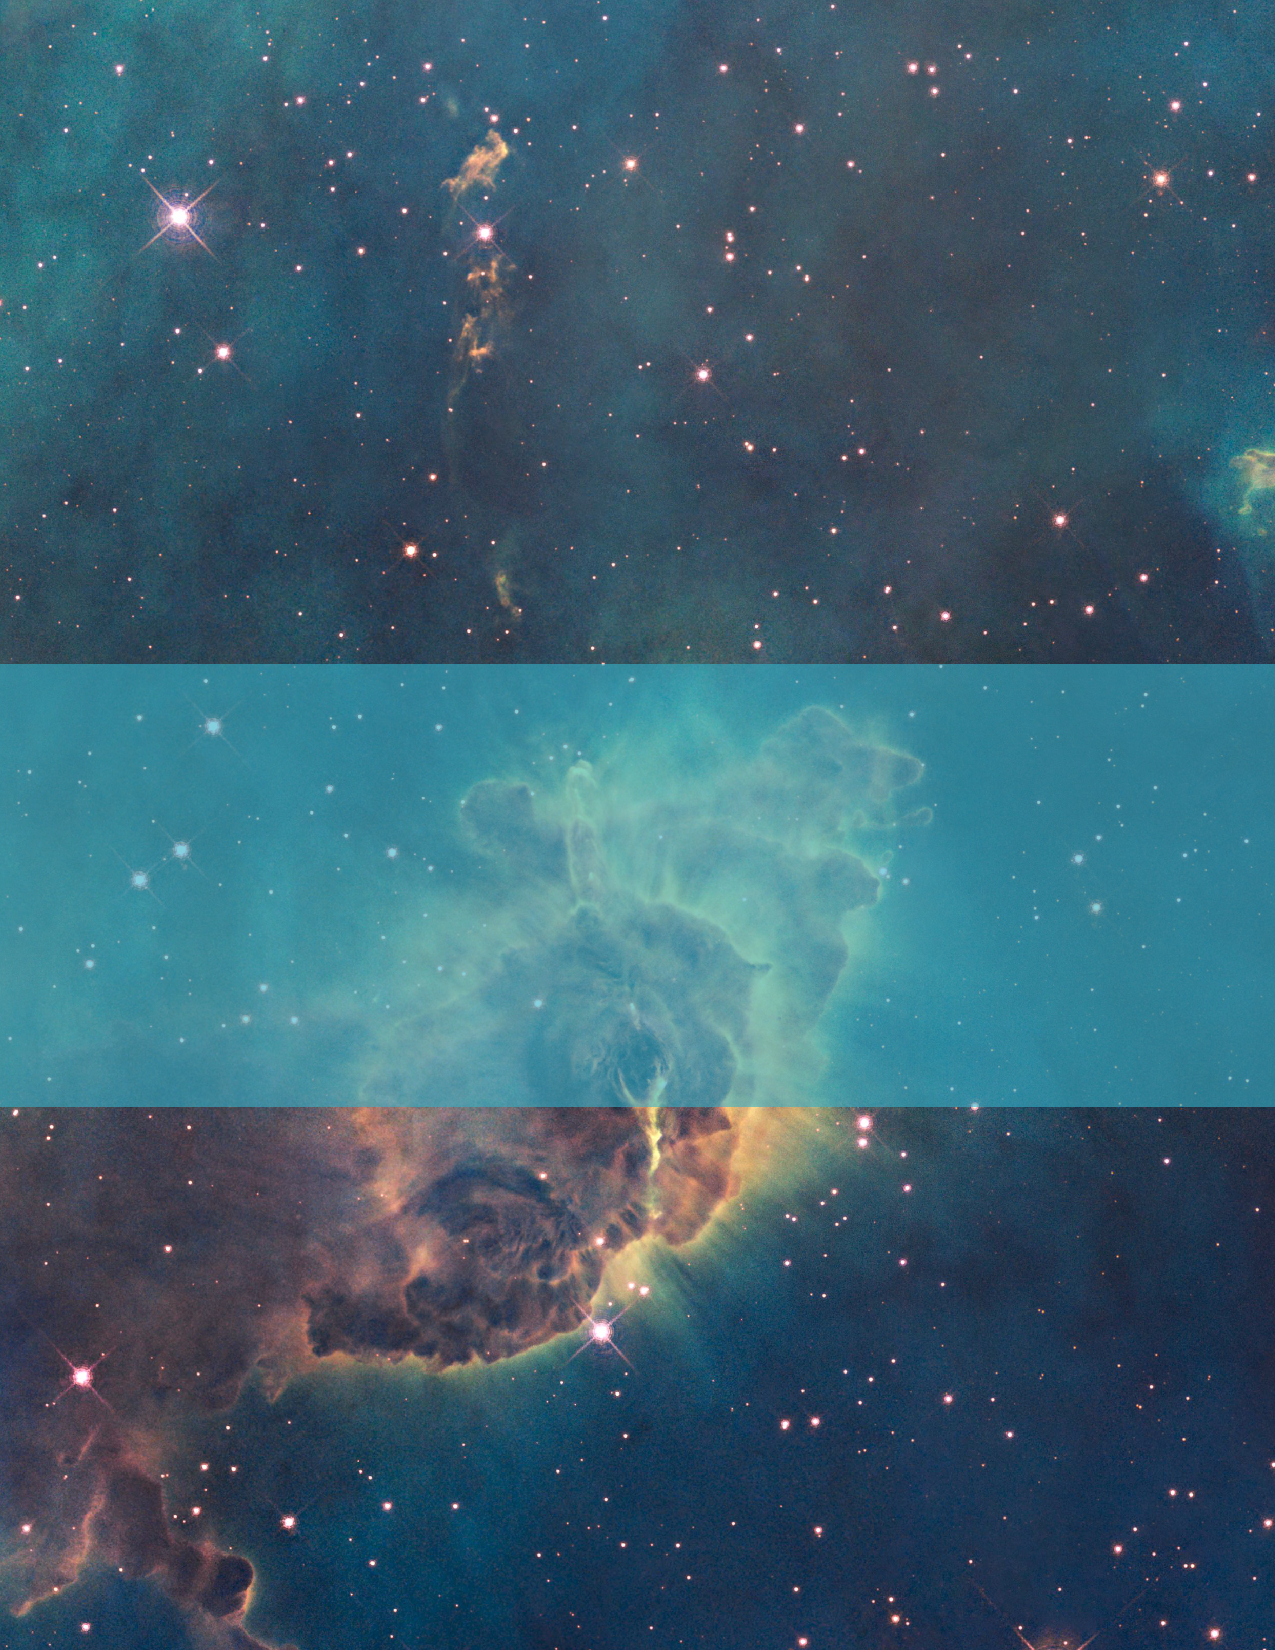
\includegraphics[scale=1.25]{esahubble}}} % Image background
\centering
\vspace*{5cm}
\par\normalfont\fontsize{35}{35}\sffamily\selectfont
\textbf{Computational Biology 2021}\\
{\LARGE Expectation-Maximization of the PMF}\par % Book title
\vspace*{1cm}
{\Huge Technical Report}\par % Author name
\endgroup

%----------------------------------------------------------------------------------------
%	COPYRIGHT PAGE
%----------------------------------------------------------------------------------------

\newpage
~\vfill
\thispagestyle{empty}

%\noindent Copyright \copyright\ 2014 Andrea Hidalgo\\ % Copyright notice

\noindent \textsc{Biosystems Simulation Lab, National Chiao Tung University}\\

\noindent \textsc{github.com/yizaochen/emtheory}\\ % URL

\noindent This research was done under the supervision of Dr. Jhih-Wei Chu with the financial support of MOST Taiwan.\\ % License information

\noindent \textit{First release, November 2020} % Printing/edition date

%----------------------------------------------------------------------------------------
%	TABLE OF CONTENTS
%----------------------------------------------------------------------------------------

\chapterimage{head1.png} % Table of contents heading image

\pagestyle{empty} % No headers

\tableofcontents % Print the table of contents itself

%\cleardoublepage % Forces the first chapter to start on an odd page so it's on the right

\pagestyle{fancy} % Print headers again

%----------------------------------------------------------------------------------------
%	CHAPTER 1
%----------------------------------------------------------------------------------------
\chapterimage{head2.png} % Chapter heading image
\chapter{Langevin Dynamics}
\section{Basic Equation}
\begin{definition}
\begin{align}
        dx_t=D F(x_t)dt  + \sqrt{2D}d{W}_t.
\end{align}
\label{langevin}
\end{definition}

\subsection{The most disordered dynamics as reference}
\begin{align}
      V_{\rm ref}(x) &= 0\\
      F_{\rm ref}(x) &= 0\\
      D &= 4.845 \times 10^{9}~~\text{\AA}^2~s^{-1}  
\end{align}

\begin{center}
        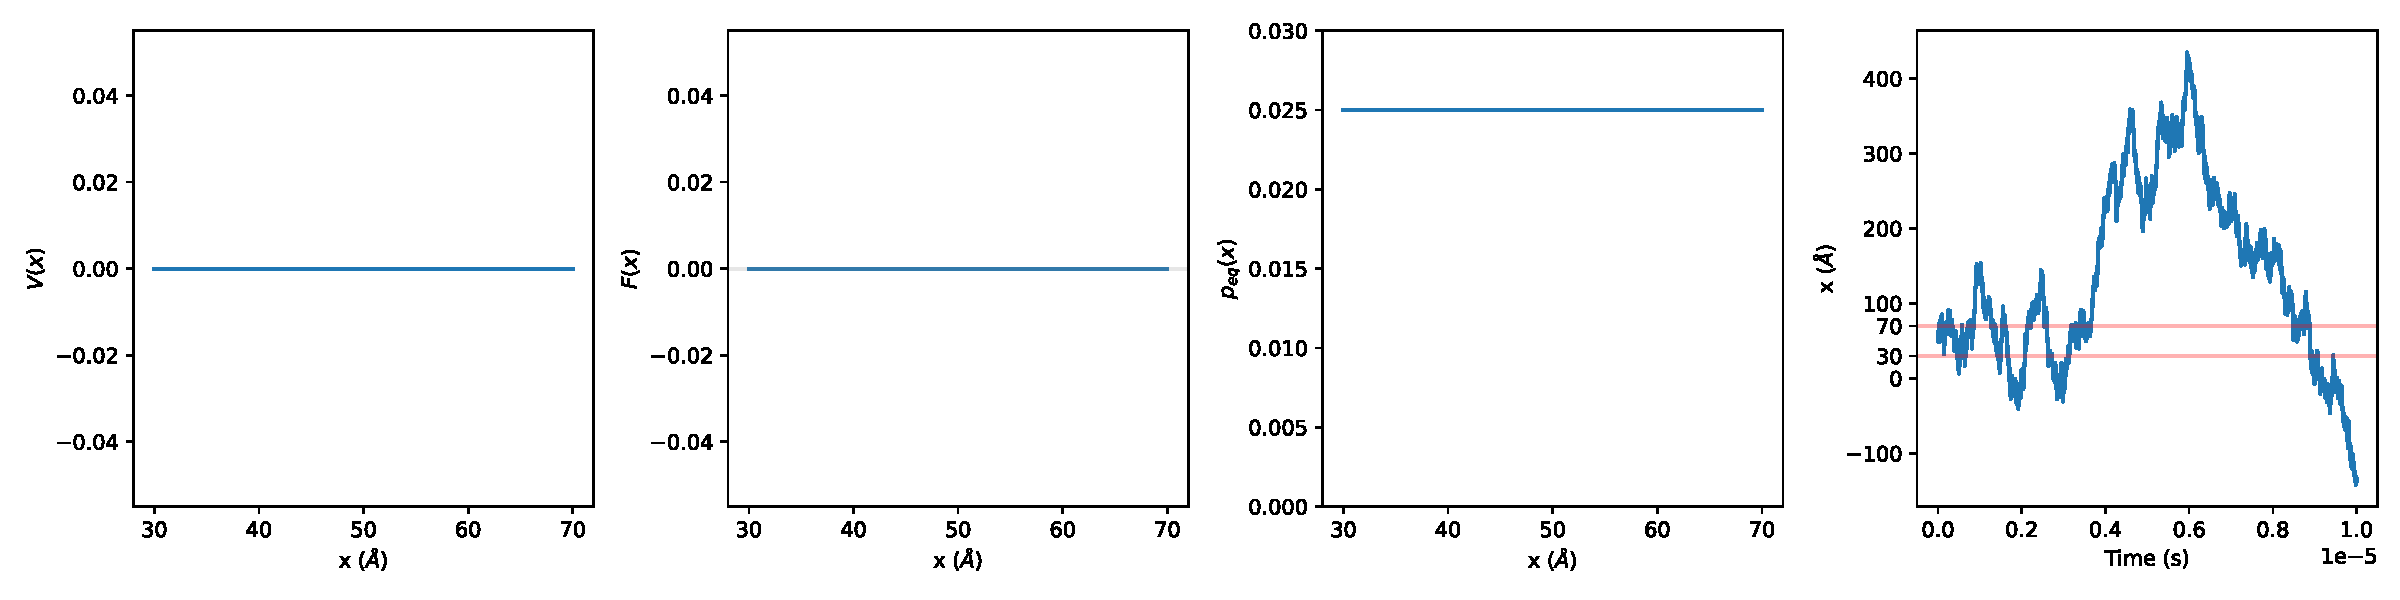
\includegraphics[scale=0.35]{ch1/zero_force_dynamic.pdf} 
\end{center}

\subsection{Harmonic Well}
\begin{align}
        V(x) &= k (x-50)^2\\
        F(x) &= 2k(x-50)  \\
        p_{\rm eq}(x) &= \exp{(-V(x))} \\
        D &= 4.845 \times 10^{9}~~\text{\AA}^2~s^{-1}
\end{align}
Here, $k=0.5$ kcal/mol/Å$^2$
\begin{center}
        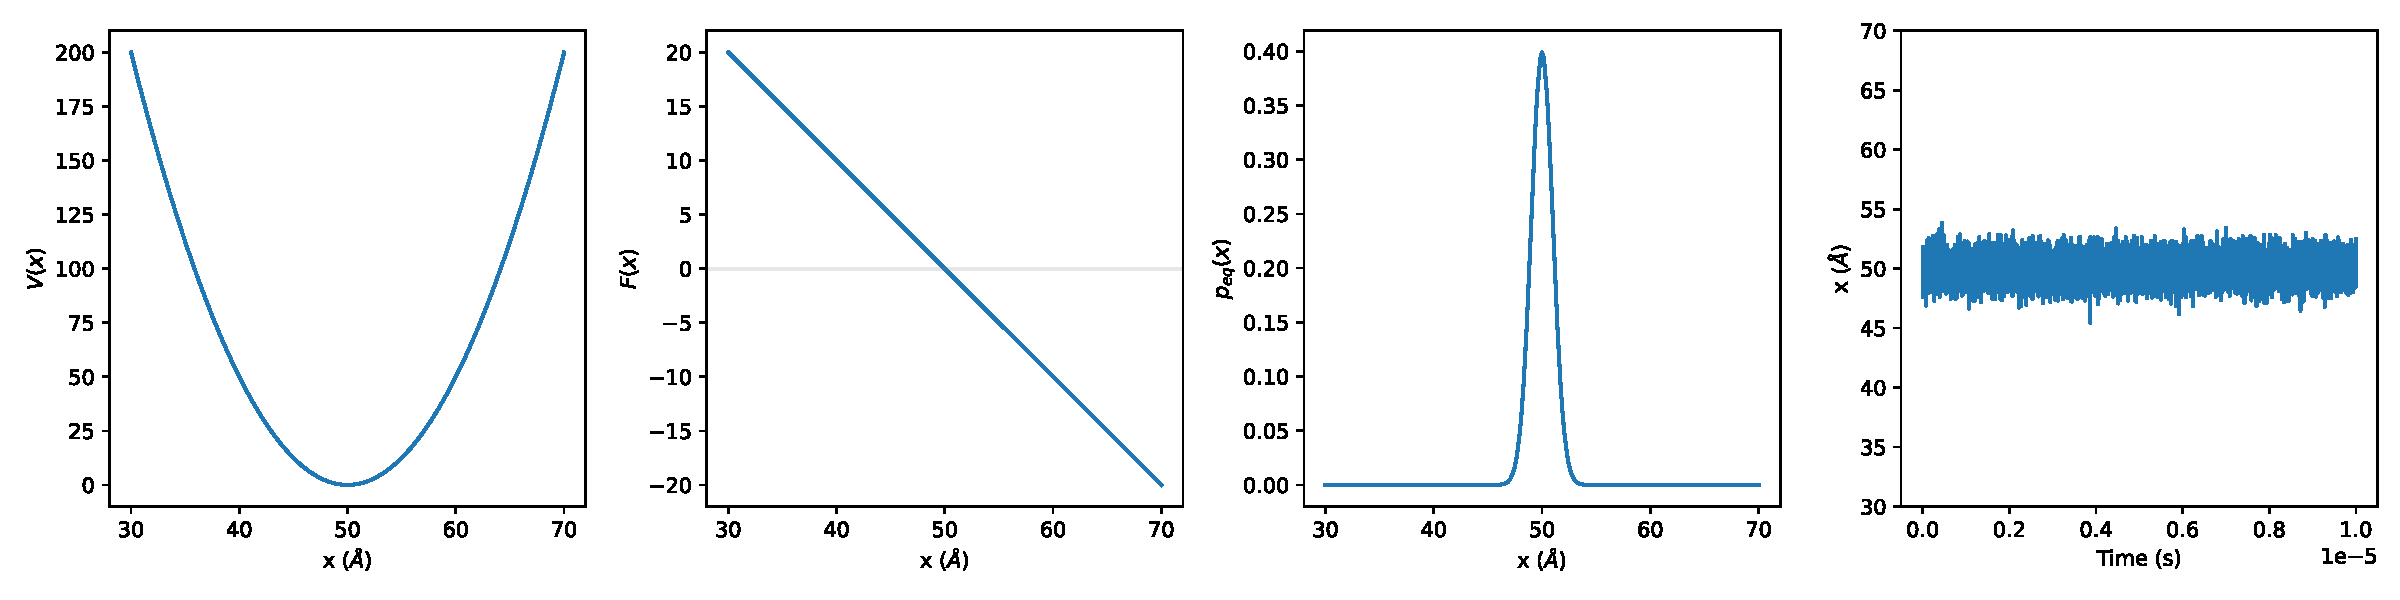
\includegraphics[scale=0.35]{ch1/single_well.pdf} 
\end{center}

\subsection{Double Well}
\begin{align}
        V(x) &= -\frac{1}{4} h^4 x^2 + \frac{1}{2} c^2 x^4 + d\\
        c    &= \sqrt{\frac{2H}{W^4}},H > 0 \\
        h    &= \sqrt{2Wc} \\
        F(x) &= \frac{1}{2} h^4 x - 2 c^2 x^3\\
        p_{\rm eq}(x) &= \exp{(-V(x))} \\
        D &= 4.845 \times 10^{9}~~\text{\AA}^2~s^{-1}\\
\end{align}
where $d$ is y-intercept, $H$ is the height of the central peak, and $W$ is the width between two valleys. In the following case, $H=5$ and $W=10$.
\begin{center}
        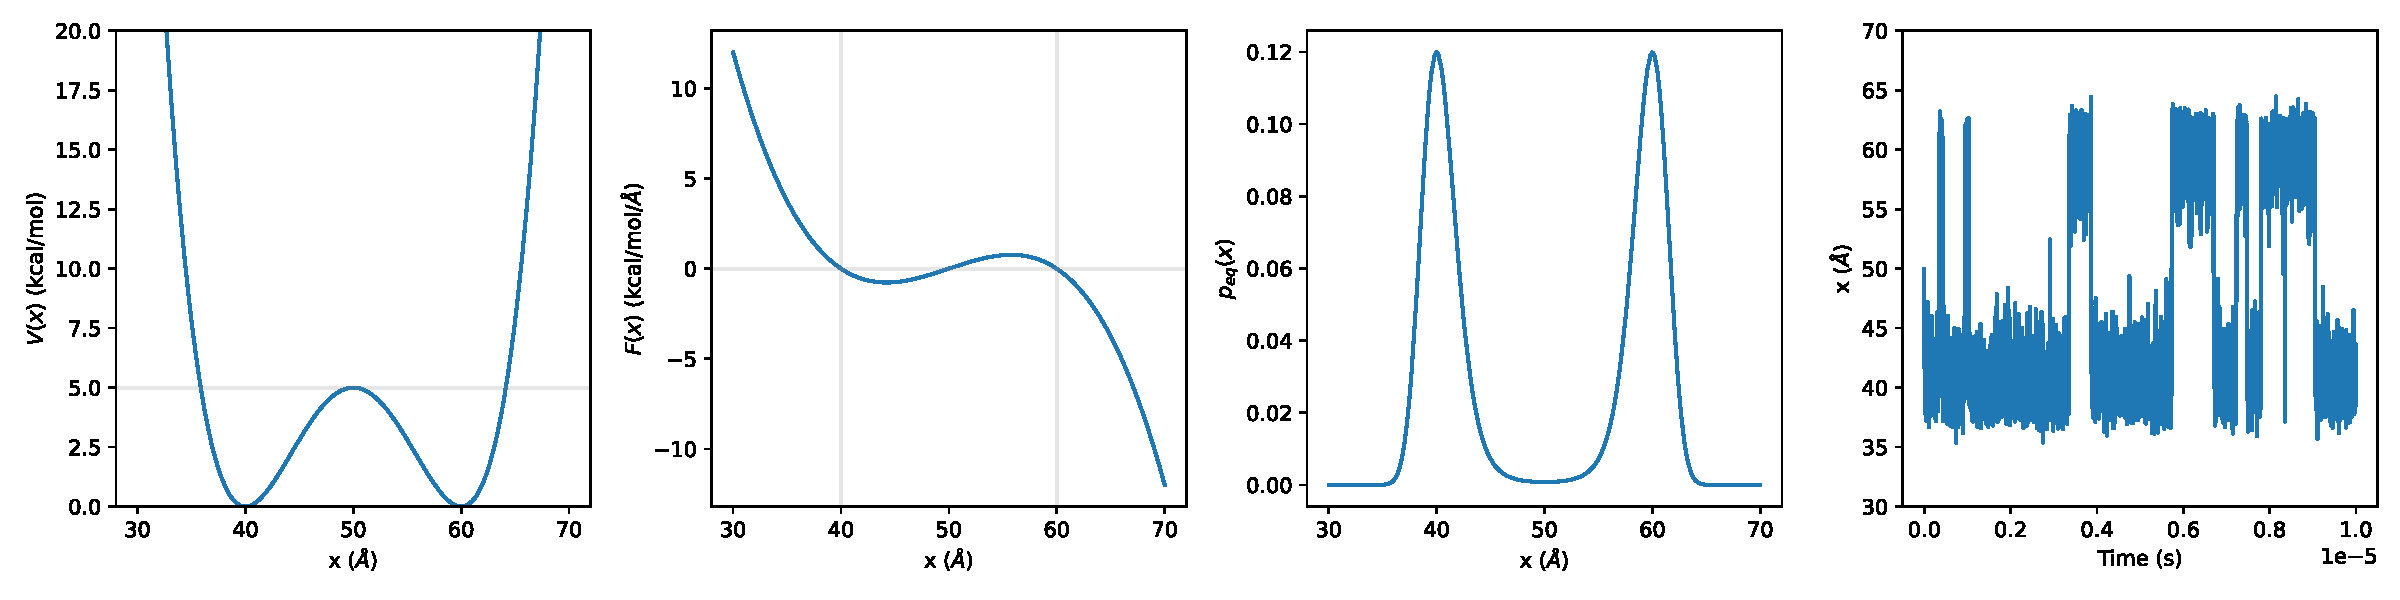
\includegraphics[scale=0.35]{ch1/double_well.pdf} 
\end{center}
%----------------------------------------------------------------------------------------
%	CHAPTER 2
%----------------------------------------------------------------------------------------
\chapterimage{head2.png} % Chapter heading image
\chapter{Hidden Markov Model}
\section{Graphical Model}
\begin{definition}
We denote a particular configuration as $(\textbf{x}, \textbf{y})$
\begin{equation}
(\textbf{x}, \textbf{y})=(x_0, x_1, \cdots, x_T, y_0, y_1, \cdots, y_T)
\end{equation}
\end{definition}

\begin{definition}[The joint probability]
\begin{equation}
p(\textbf{x}, \textbf{y})= p(x_0)\prod_{t=0}^{T-1} p(x_{t+1}|x_t) \prod_{t=0}^{T}p(y_t|x_t)
\end{equation}
\end{definition}
\begin{center}
        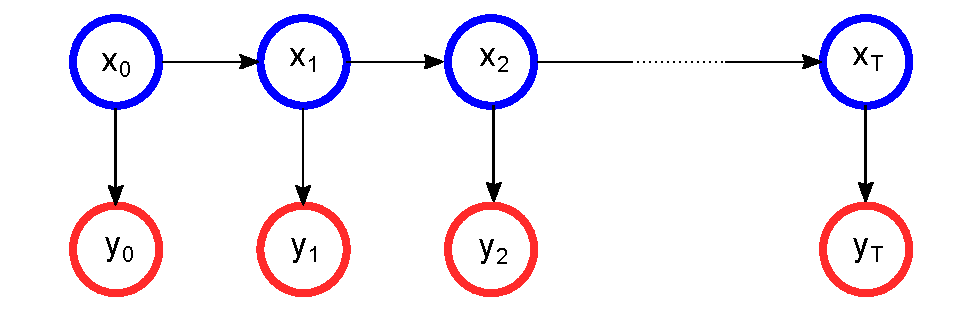
\includegraphics[scale=0.8]{ch2/graphical.pdf}   
\end{center}

\section{Log-likelihood}
We will use the following four states model to illustrate how we calculate the log-likelihood.
\begin{center}
        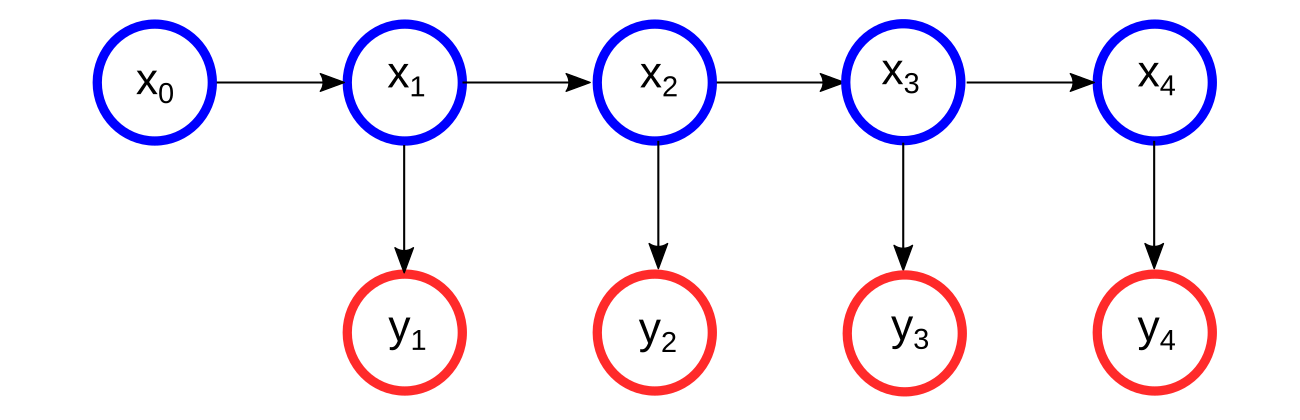
\includegraphics[scale=0.8]{ch2/four_states_ex.png}   
\end{center}

\begin{definition}[$\left< \hat{\alpha}_{t_0} \right|$]
Since there is no external forces, the initial state, $\left< \hat{\alpha}_{t_0} \right|$, is assumed to follow the equilibrium distribution $\rho_{eq}(x)=\sqrt{p_{eq}(x)}$, that is
\begin{equation}
        \left< \alpha_{t_0} | x \right> = \rho_{eq}(x)
\end{equation}
\begin{center}
        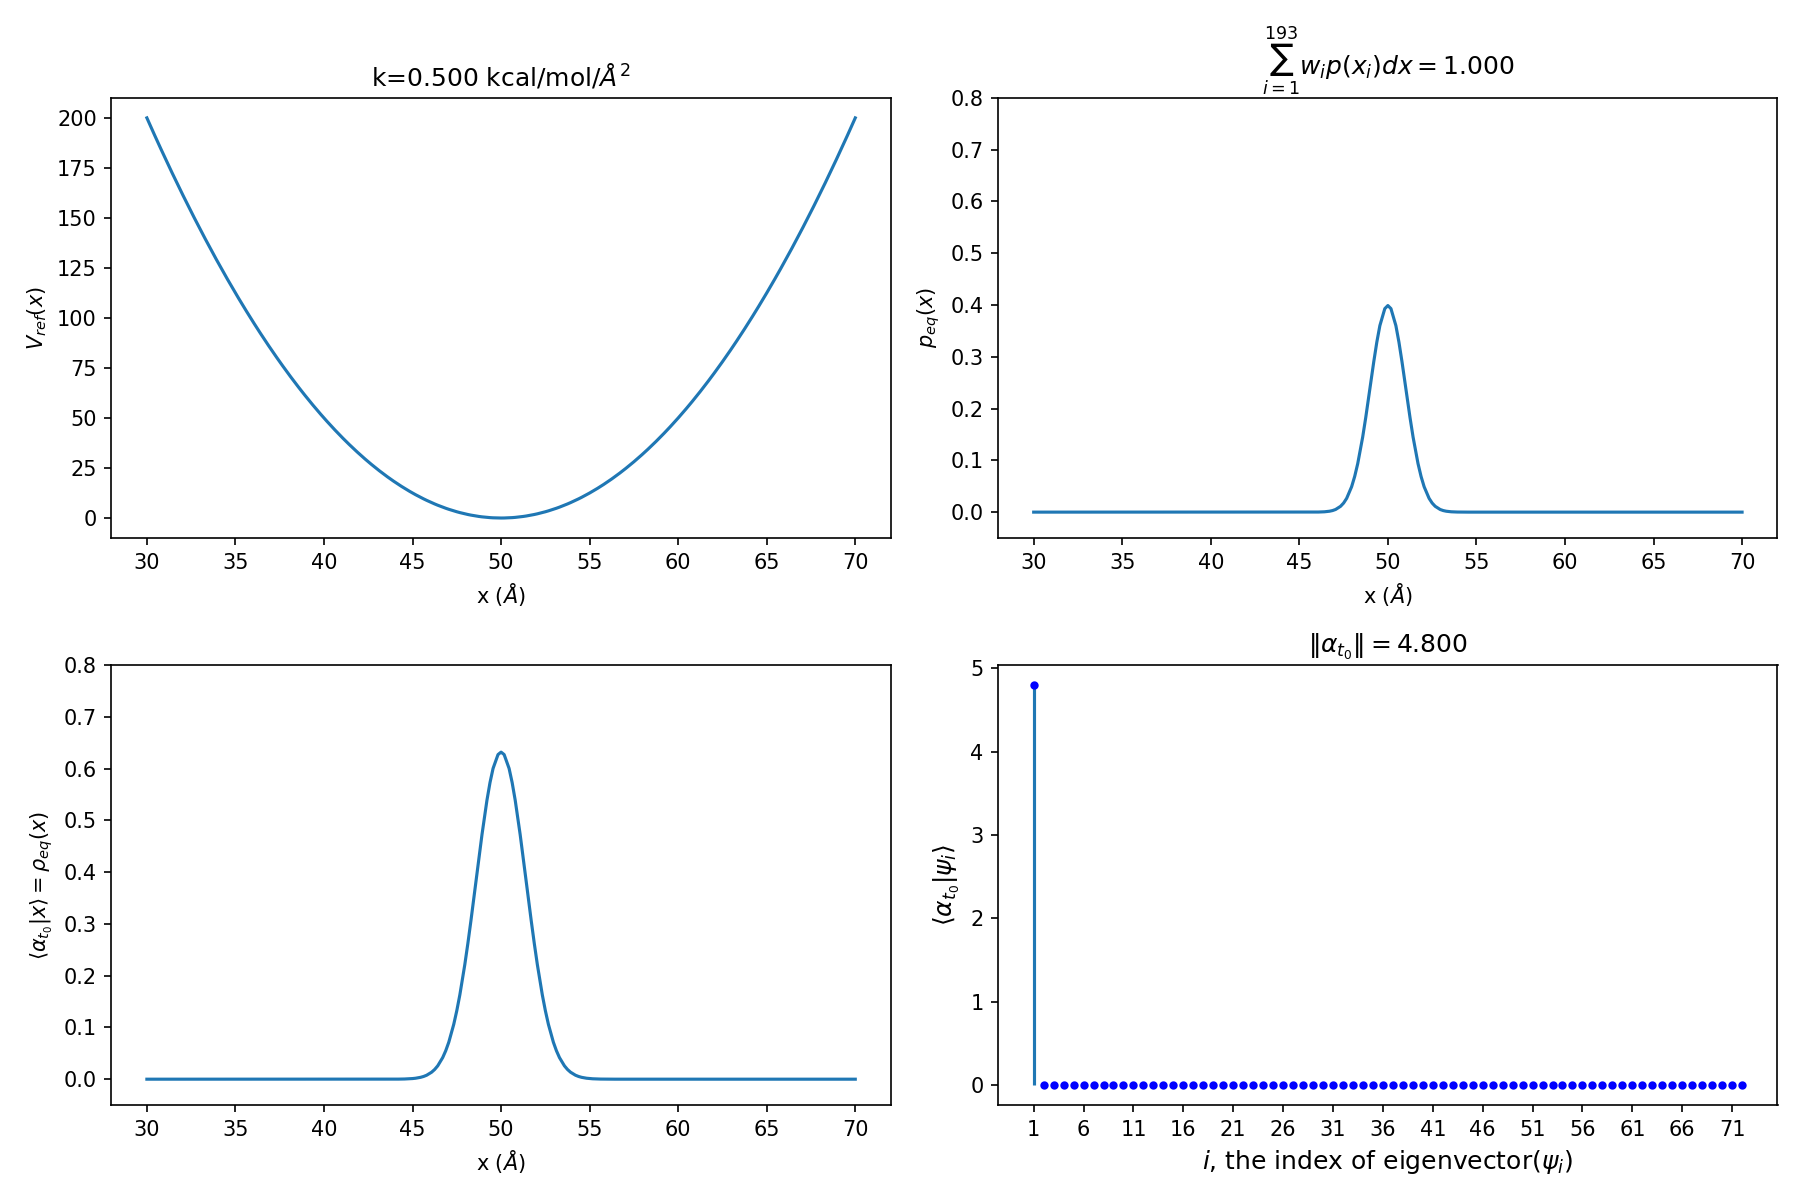
\includegraphics[scale=0.45]{ch2/alpha_t0.png}   
\end{center}
And we know
\begin{align*}
        p(x,t=0) &= \rho_{eq}(x) \rho_{eq}(x)\\
        &= \rho_{eq}(x)[a_{1}(0) \psi_1(x)+a_{2}(0)\psi_2(x)+\cdots+a_{72}(0)\psi_{72}(x)]       
\end{align*}
$\left< \alpha_{t_0} \right|$ is a vector, which is shown in the right-bottom figure.
\begin{equation}
        \left< \alpha_{t_0} \right| = \begin{bmatrix}\left< \alpha_{t_0} | \psi_1 \right> & \left< \alpha_{t_0} | \psi_2 \right> & \cdots & \left< \alpha_{t_0} | \psi_{72} \right> \end{bmatrix}
\end{equation}
and the norm of $\left< \alpha_{t_0} \right|$
\begin{equation}
        \norm{\alpha_{t_0}} = \sqrt{a_{1}^2(0) + a_{2}^2(0) + \cdots + a_{36}^2(0)}       
\end{equation}
Furthermore, note that
\begin{equation}
        \left< \hat{\alpha}_{t_0} \right| = \frac{\left< \alpha_{t_{0}} \right|}{\norm{\alpha_{t_{0}}}} = \left< \alpha_{t_{0}} \right|
\end{equation}
because $\norm{\alpha_{t_0}} = 1$
\end{definition}

\begin{definition}[$\rho(x, t=\Delta t) = \left<\alpha_{t_0}| e^{-\textbf{H}\Delta t}|x \right>$]
\begin{align*}
        &p(x,t=\Delta t) = \rho_{eq}(x) \rho(x, \Delta t)\\
        &= \rho_{eq}(x)[a_{1}(0) \exp{(-\lambda_{1}\Delta t)}\psi_1(x)+a_{2}(0)\exp{(-\lambda_{2}\Delta t)}\psi_2(x)+\cdots+a_{72}(0)\exp{(-\lambda_{72}\Delta t)}\psi_{72}(x)]  \\
        &=  \rho_{eq}(x)[a_{1}(0)\psi_1(x)+a_{2}(0)\exp{(-\lambda_{2}\Delta t)}\psi_2(x)+\cdots+a_{72}(0)\exp{(-\lambda_{72}\Delta t)}\psi_{72}(x)]  
\end{align*}
where $\lambda_1 = 0$
\end{definition}

\begin{definition}[$\left< \hat{\alpha}_{t_1}\right|$]
\begin{equation}
        \left< \alpha_{t_1} \right| = \left< \alpha_{t_0} \right| e^{-\textbf{H} \Delta t} \textbf{y}_1     
\end{equation}
\begin{equation}
        \left< \hat{\alpha}_{t_1} \right| = \frac{\left< \alpha_{t_0} \right| e^{-\textbf{H}\Delta t} \textbf{y}_1}{\norm{\left< \alpha_{t_0} \right| e^{-\textbf{H}\Delta t} \textbf{y}_1}} = \frac{\left< \alpha_{t_{1}} \right|}{\norm{\alpha_{t_{1}}}}
\end{equation}
\begin{center}
        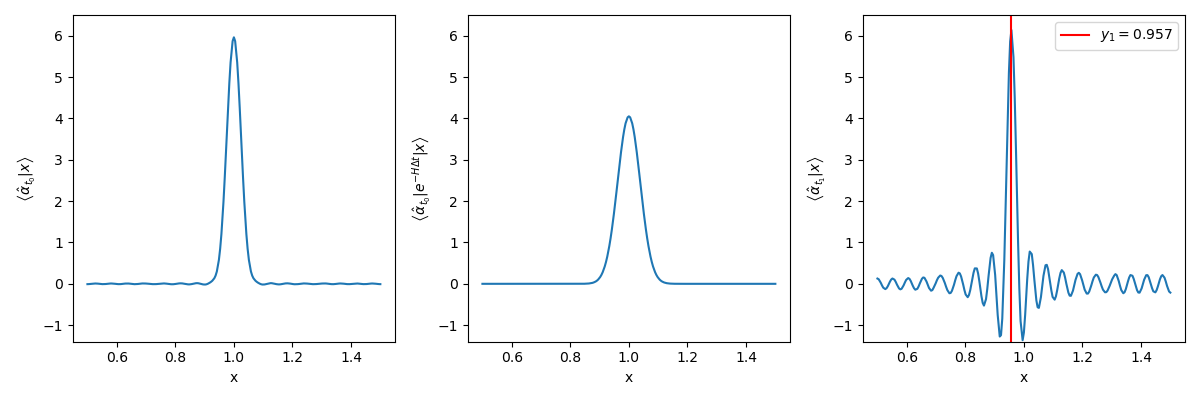
\includegraphics[scale=0.3]{ch2/alpha_1.png}   
\end{center}
\end{definition}

\begin{definition}[$\left< \hat{\alpha}_{t_2}\right|$]
\begin{equation}
        \left< \alpha_{t_2} \right| = \left< \alpha_{t_1} \right| e^{-\textbf{H}\Delta t} \textbf{y}_2     
\end{equation}
\begin{equation}
        \left< \hat{\alpha}_{t_2} \right| 
	= \frac{\left< \hat{\alpha}_{t_1} \right| e^{-\textbf{H}\Delta t} \textbf{y}_2}{\norm{\left< \hat{\alpha}_{t_1} \right| e^{-\textbf{H}\Delta t} \textbf{y}_2}} 
	= \frac{1}{\norm{\alpha_{t_{1}}}} \frac{\left< \alpha_{t_1} \right| e^{-\textbf{H}\Delta t} \textbf{y}_2}{\norm{\left< \hat{\alpha}_{t_1} \right| e^{-\textbf{H}\Delta t} \textbf{y}_2}} 
	= \frac{1}{\norm{\alpha_{t_{1}}}} \frac{1}{\norm{\left< \hat{\alpha}_{t_1} \right| e^{-\textbf{H}\Delta t} \textbf{y}_2}} \left< \alpha_{t_2} \right| 
	= \frac{1}{\norm{\alpha_{t_2}}} \left< \alpha_{t_2} \right|
\end{equation}
where
\begin{equation}
        \norm{\alpha_{t_2}} = \norm{\alpha_{t_{1}}} \norm{\left< \hat{\alpha}_{t_1} \right| e^{-\textbf{H}\Delta t} \textbf{y}_2} 
	= \norm{\left < \hat{\alpha}_{t_{0}} \right| e^{-\textbf{H}\Delta t} \textbf{y}_1} \norm{\left< \hat{\alpha}_{t_1} \right| e^{-\textbf{H}\Delta t} \textbf{y}_2}
\end{equation}
\begin{center}
        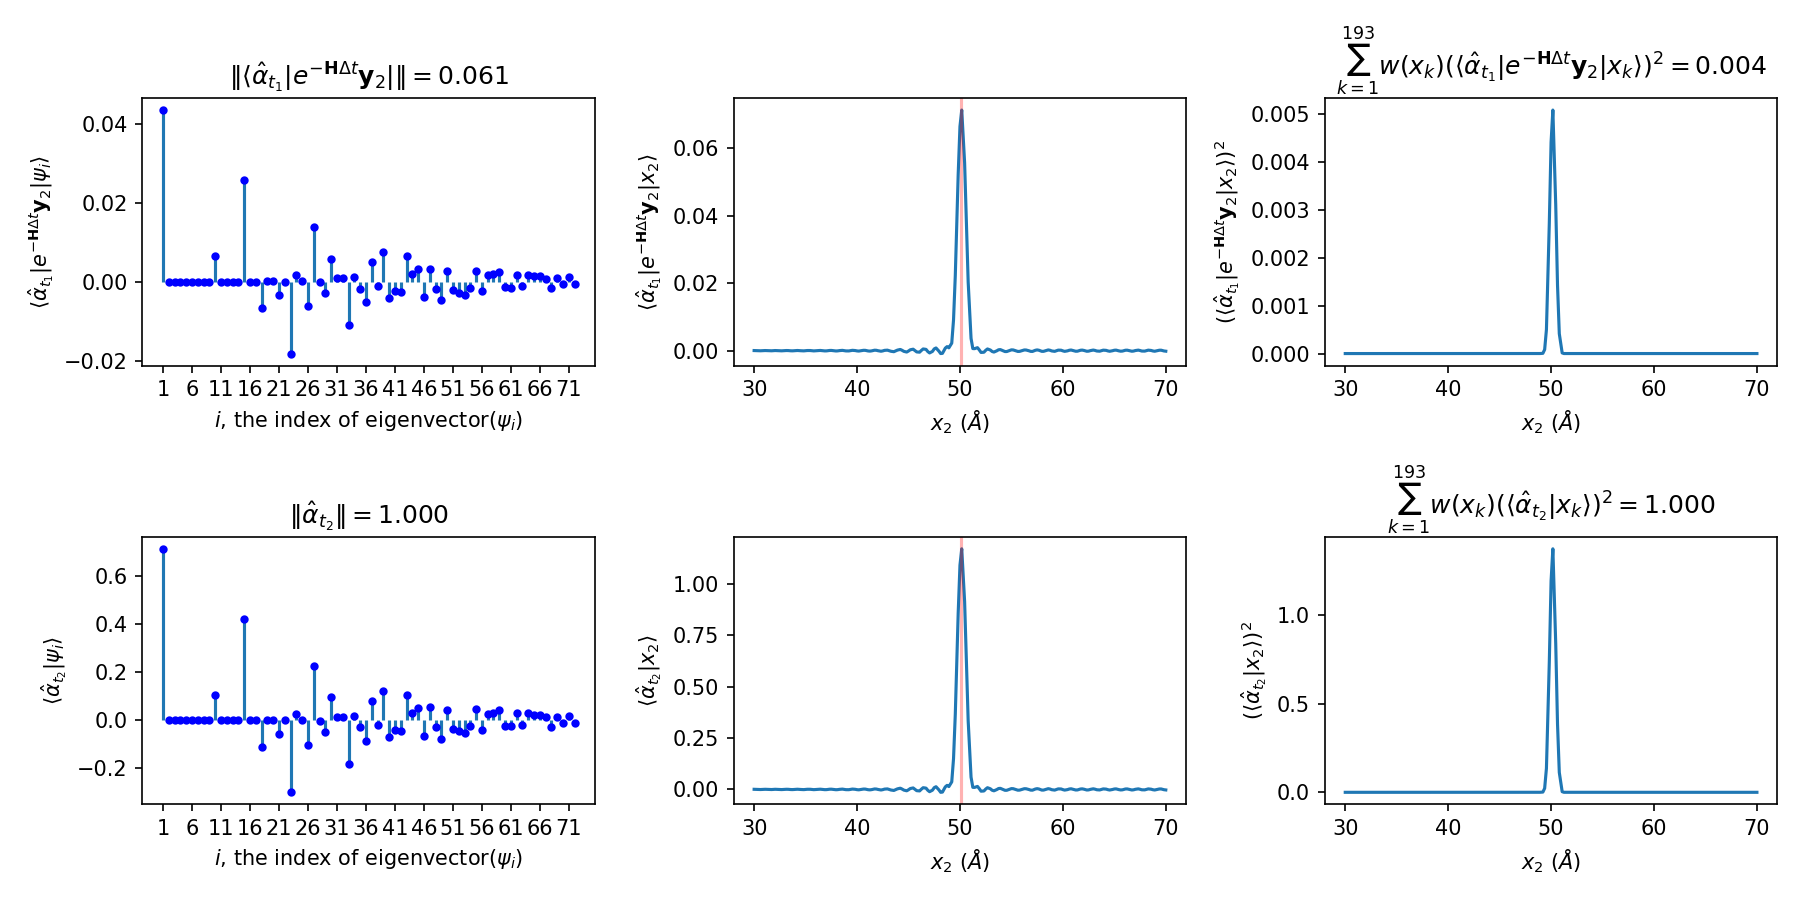
\includegraphics[scale=0.3]{ch2/alpha_2.png}   
\end{center}
\end{definition}

\begin{definition}[$\left< \hat{\alpha}_{t_3}\right|$]
\begin{equation}
        \left< \alpha_{t_3} \right| = \left< \alpha_{t_2} \right| e^{-\textbf{H}\Delta t} \textbf{y}_3               
\end{equation}
\begin{equation}
        \left< \hat{\alpha}_{t_3} \right| 
	= \frac{\left< \hat{\alpha}_{t_2} \right| e^{-\textbf{H}\Delta t} \textbf{y}_3}{\norm{\left< \hat{\alpha}_{t_2} \right| e^{-\textbf{H}\Delta t} \textbf{y}_3}} 
	= \frac{1}{\norm{\alpha_{t_{2}}}} \frac{\left< \alpha_{t_2} \right| e^{-\textbf{H}\Delta t} \textbf{y}_3}{\norm{\left< \hat{\alpha}_{t_2} \right| e^{-\textbf{H}\Delta t} \textbf{y}_3}} 
	= \frac{1}{\norm{\alpha_{t_3}}} \left< \alpha_{t_3} \right|
\end{equation}
where
\begin{equation}
        \norm{\alpha_{t_3}} = \norm{\alpha_{t_{2}}} \norm{\left< \hat{\alpha}_{t_2} \right| e^{-\textbf{H}\Delta t} \textbf{y}_3} 
        = \norm{\left < \hat{\alpha}_{t_{0}} \right| e^{-\textbf{H}\Delta t} \textbf{y}_1} \norm{\left< \hat{\alpha}_{t_1} \right| e^{-\textbf{H}\Delta t} \textbf{y}_2} \norm{\left < \hat{\alpha}_{t_{2}} \right| e^{-\textbf{H}\Delta t} \textbf{y}_3}    
\end{equation}
\begin{center}
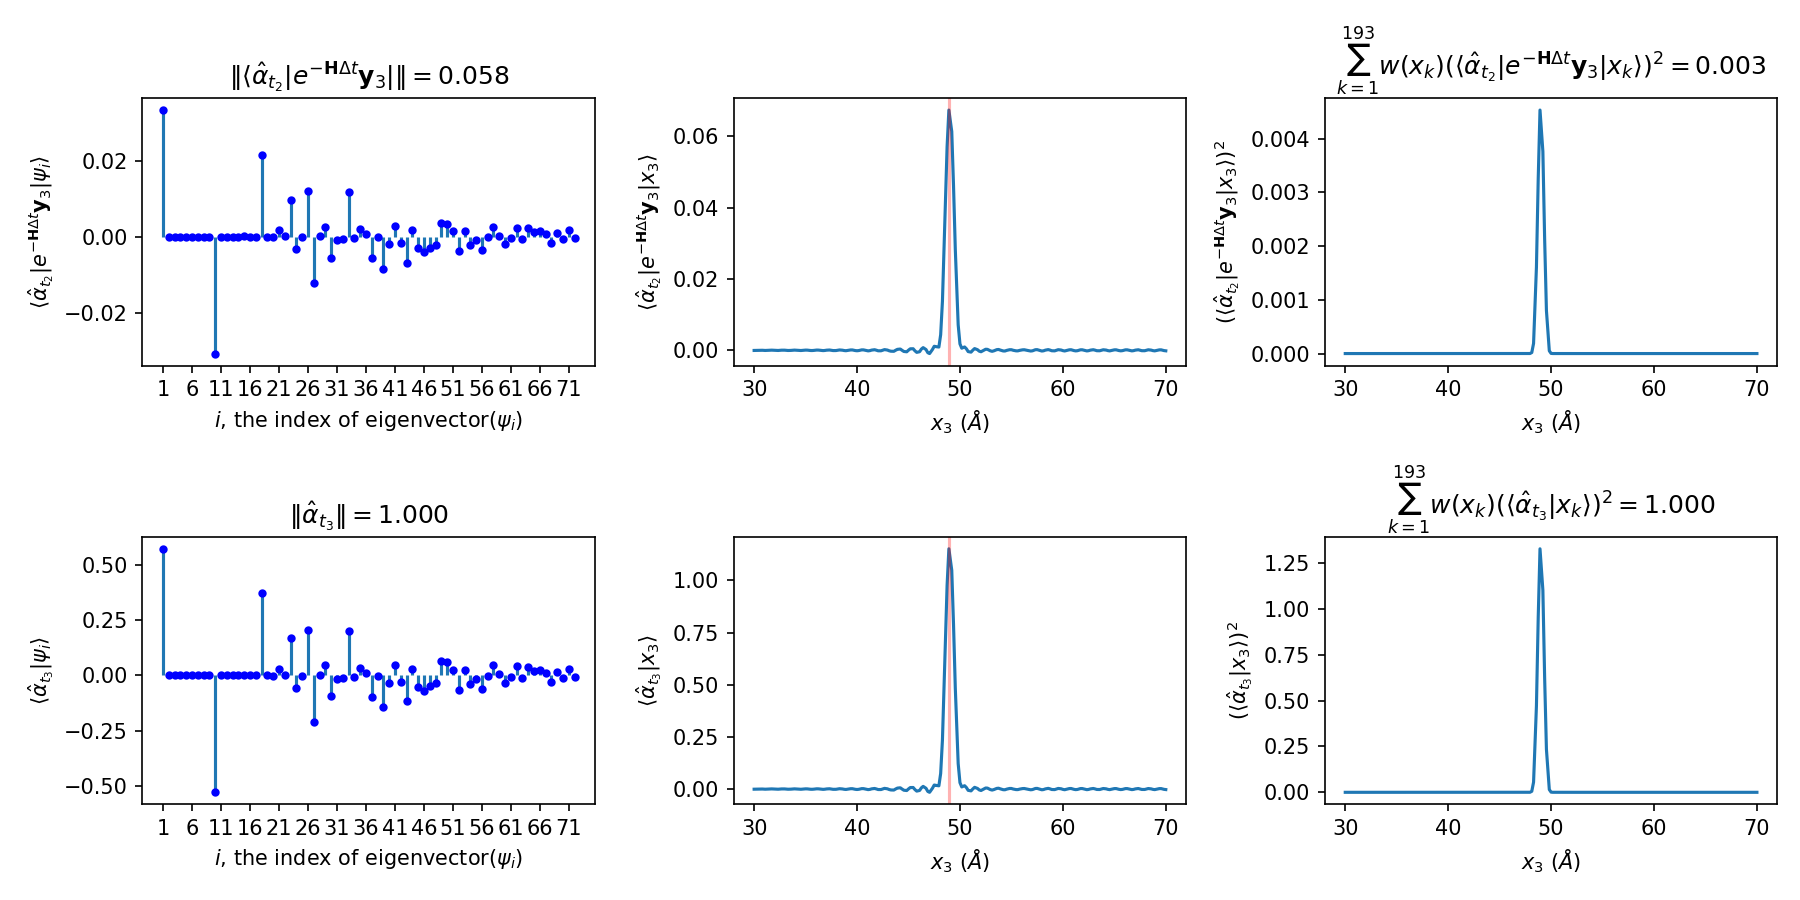
\includegraphics[scale=0.3]{ch2/alpha_3.png}
\end{center}
\end{definition}

\begin{definition}[$\left< \hat{\alpha}_{t_4}\right|$]
\begin{equation}
        \left< \alpha_{t_4} \right| = \left< \alpha_{t_3} \right| e^{-\textbf{H}\Delta t} \textbf{y}_4
\end{equation}
\begin{equation}
        \left< \hat{\alpha}_{t_4} \right| 
	= \frac{\left< \hat{\alpha}_{t_3} \right| e^{-\textbf{H}\Delta t} \textbf{y}_4}{\norm{\left< \hat{\alpha}_{t_3} \right| e^{-\textbf{H}\Delta t} \textbf{y}_4}} 
        = \frac{1}{\norm{\alpha_{t_{3}}}} \frac{\left< \alpha_{t_3} \right| e^{-\textbf{H}\Delta t} \textbf{y}_4}{\norm{\left< \hat{\alpha}_{t_3} \right| e^{-\textbf{H}\Delta t} \textbf{y}_4}} 
        = \frac{1}{\norm{\alpha_{t_4}}} \left< \alpha_{t_4} \right|
\end{equation}
where
\begin{align*}
        \norm{\alpha_{t_4}} &= \norm{\alpha_{t_{3}}} \norm{\left< \hat{\alpha}_{t_3} \right| e^{-\textbf{H}\Delta t} \textbf{y}_4}\\
	&= \norm{\left < \hat{\alpha}_{t_{0}} \right| e^{-\textbf{H}\Delta t} \textbf{y}_1} \norm{\left< \hat{\alpha}_{t_1} \right| e^{-\textbf{H}\Delta t} \textbf{y}_2} \norm{\left < \hat{\alpha}_{t_{2}} \right| e^{-\textbf{H}\Delta t} \textbf{y}_3} \norm{\left < \hat{\alpha}_{t_{3}} \right| e^{-\textbf{H}\Delta t} \textbf{y}_4}
\end{align*}
\begin{center}
        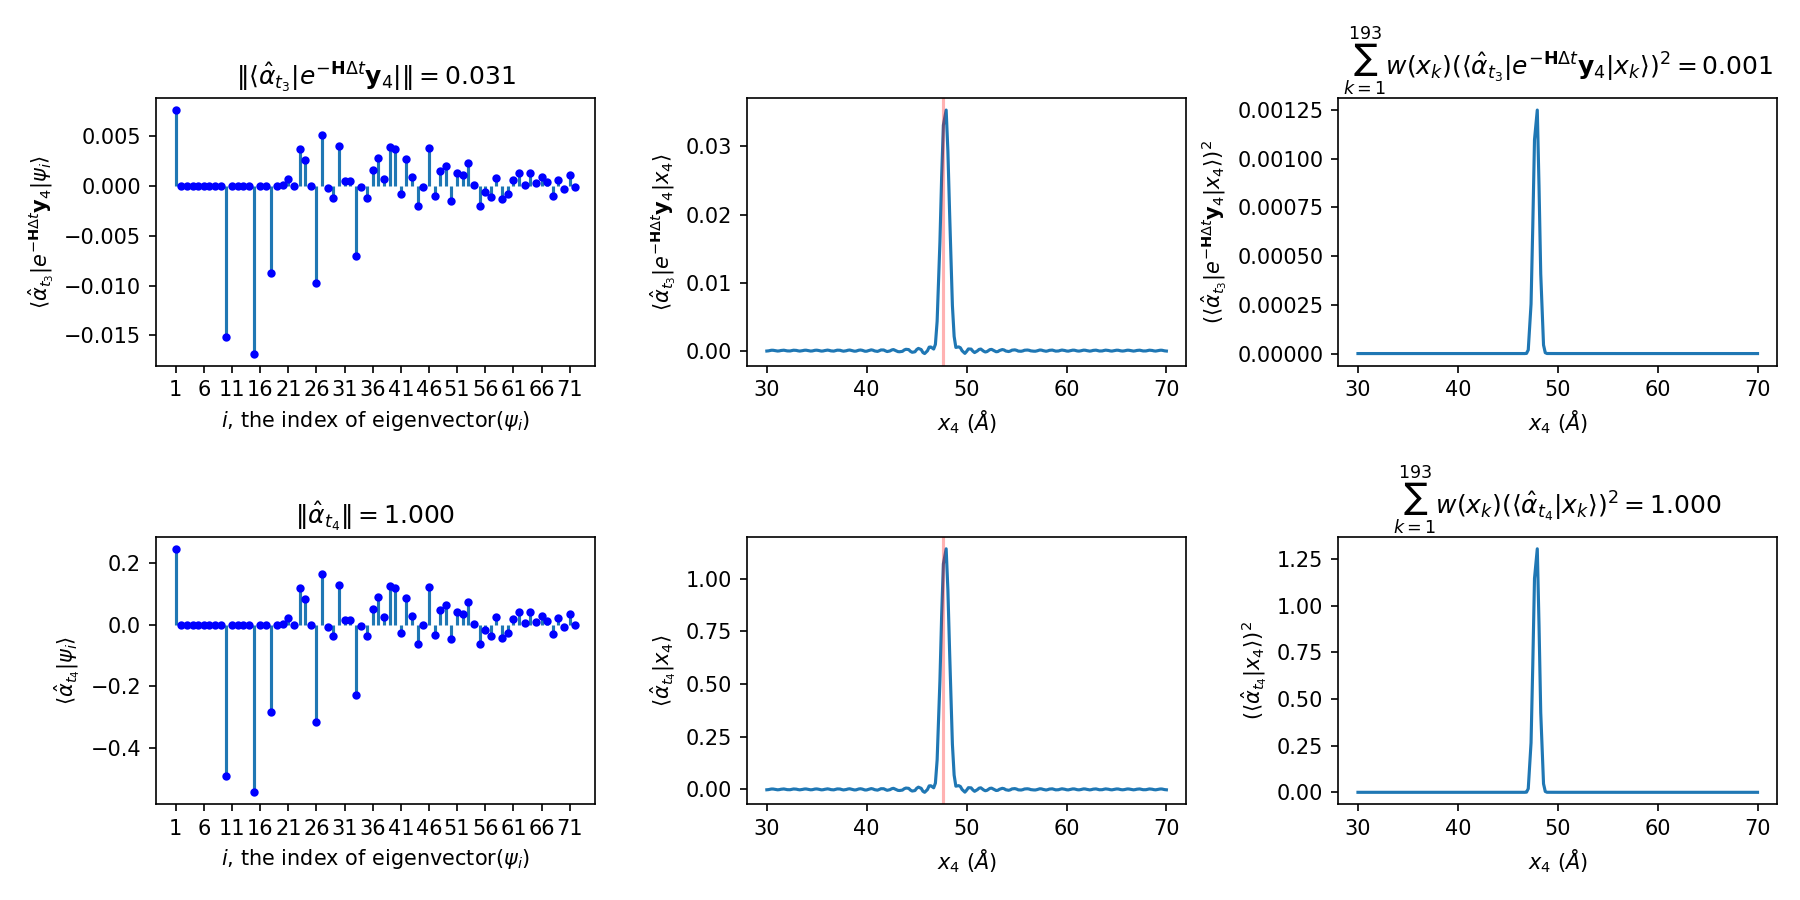
\includegraphics[scale=0.3]{ch2/alpha_4.png}
\end{center}
\end{definition}

\begin{definition}[$\left | \hat{\beta}_{t_4} \right > $]
And the final one is
\begin{center}
        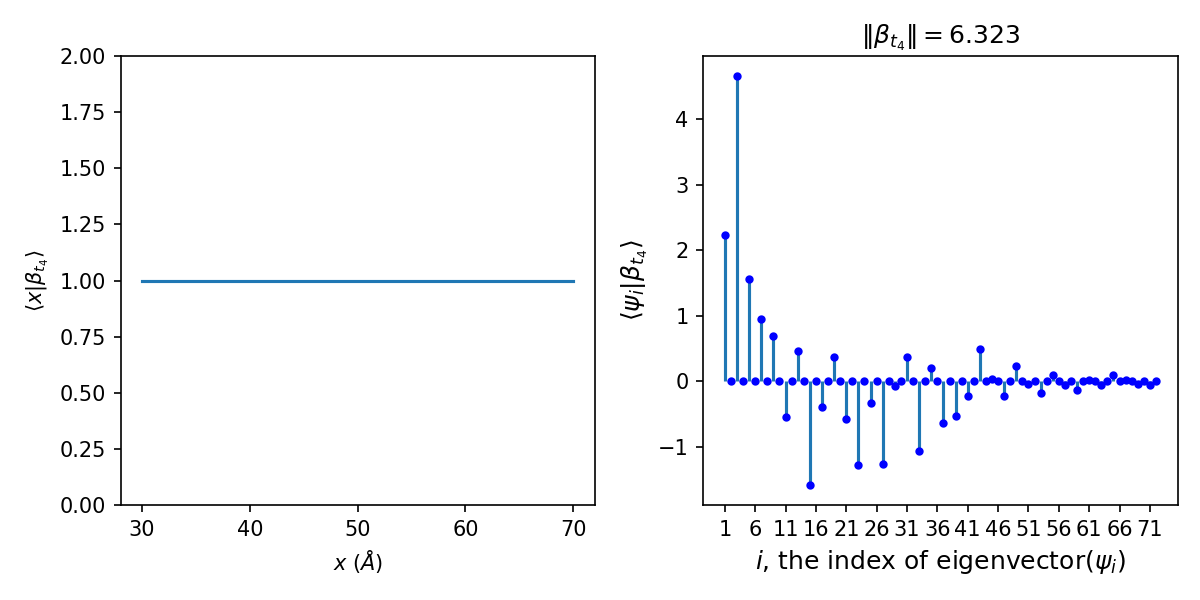
\includegraphics[scale=0.3]{ch2/beta_4.png}
\end{center}
\end{definition}

\begin{definition}[Likelihood functional]
\begin{align*}
        \mathcal{P}(Y(t) ; F(x),D) &= \mathcal{P}(Y(t) ; \theta)= \mathcal{L}[\theta] \\
	&= \langle \alpha_{t_0} |e^{-\textbf{H}\Delta t_1}\textbf{y}_1e^{-\textbf{H}\Delta t_2}\textbf{y}_2 e^{-\textbf{H}\Delta t_{3}}\textbf{y}_{3} e^{-\textbf{H}\Delta t_{4}}\textbf{y}_{4} | \beta_{t_{4}} \rangle \\
	&=  \left < \alpha_{t_{4}} | \beta_{t_{4}} \right > = \norm{\alpha_{t_{4}}} \left < \hat{\alpha}_{t_{4}} | \beta_{t_{4}} \right > 
\end{align*}
\end{definition}

\begin{definition}[Log-likelihood functional]
\begin{align*}
        \ell[\theta] &= \ln \mathcal{L}[\theta] = \ln{\norm{\alpha_{t_{4}}}} + \ln{\left < \hat{\alpha}_{t_{4}} | \beta_{t_{4}} \right >} \\  
        & =2 \sum_{i=1}^{4} \ln{\frac{\norm{\alpha_{t_{i}}}}{\norm{\alpha_{t_{i-1}}}}} + \ln{\frac{ \left < \alpha_{t_{4}} | \beta_{t_{4}}\right>}{\norm{\alpha_{t_{4}}}}} \\ 
        & = 2 \sum_{i=1}^{4} \ln{\norm{\left< \hat{\alpha}_{t_{i-1}} \right| e^{-\textbf{H}\Delta t} \textbf{y}_i}} + \ln{\left < \hat{\alpha}_{t_{4}} | \beta_{t_{4}} \right >} 
\end{align*}
\end{definition}
%----------------------------------------------------------------------------------------
%	CHAPTER 3
%----------------------------------------------------------------------------------------
\chapterimage{head2.png} % Chapter heading image
\chapter{Spectral Finite Element Method}
\section{Domain of sFEM}
The grid size is 0.6250 Å. (The distance between two red points). Totally, there are 193 points.
\begin{center}
        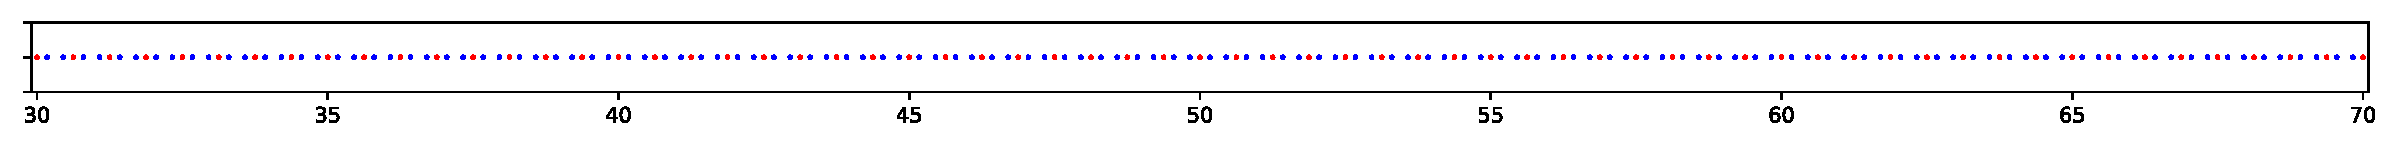
\includegraphics[scale=0.3]{ch3/node.pdf}
\end{center}
\begin{itemize}
        \item The number of spectral element, $N_h=64$
        \item The order of interpolation polynomial, $N_p=4$
\end{itemize}
Therefore, we now have $V$, a vector space  of dimension $193$. This vector space has a natural basis, or we called it the standard basis
\begin{equation}
        \{\textbf{e}_1, \textbf{e}_2, ..., \textbf{e}_{193}\}
\end{equation}
where
\begin{equation}
\textbf{e}_1=  \begin{bmatrix} 1 \\ 0 \\ \vdots \\ 0 \end{bmatrix}~~
\textbf{e}_2=  \begin{bmatrix} 0 \\ 1 \\ \vdots \\ 0 \end{bmatrix}~~
\cdots ~~
\textbf{e}_{193} = \begin{bmatrix} 0 \\ 0 \\ \vdots \\ 1 \end{bmatrix} 
\end{equation}

\section{Weight function, orthogonality and norm}
\begin{definition}[inner product]
By using integral calculus, it is common to use the following to define the inner product of two functions $f$ and $g$ with respect to a nonnegative weight function $w$ over an interval $[a, b]$:
\begin{equation}
        \langle f, g\rangle_w = \int_a^b f(x)g(x)w(x)\,dx \approx \sum_{i=1}^{193}w(x_i)f(x_i)g(x_i) 
\end{equation}
\end{definition}

\begin{definition}[weight function $w(x)$]
From the  Gauss-Lobatto quadrature, we have
\begin{center}
        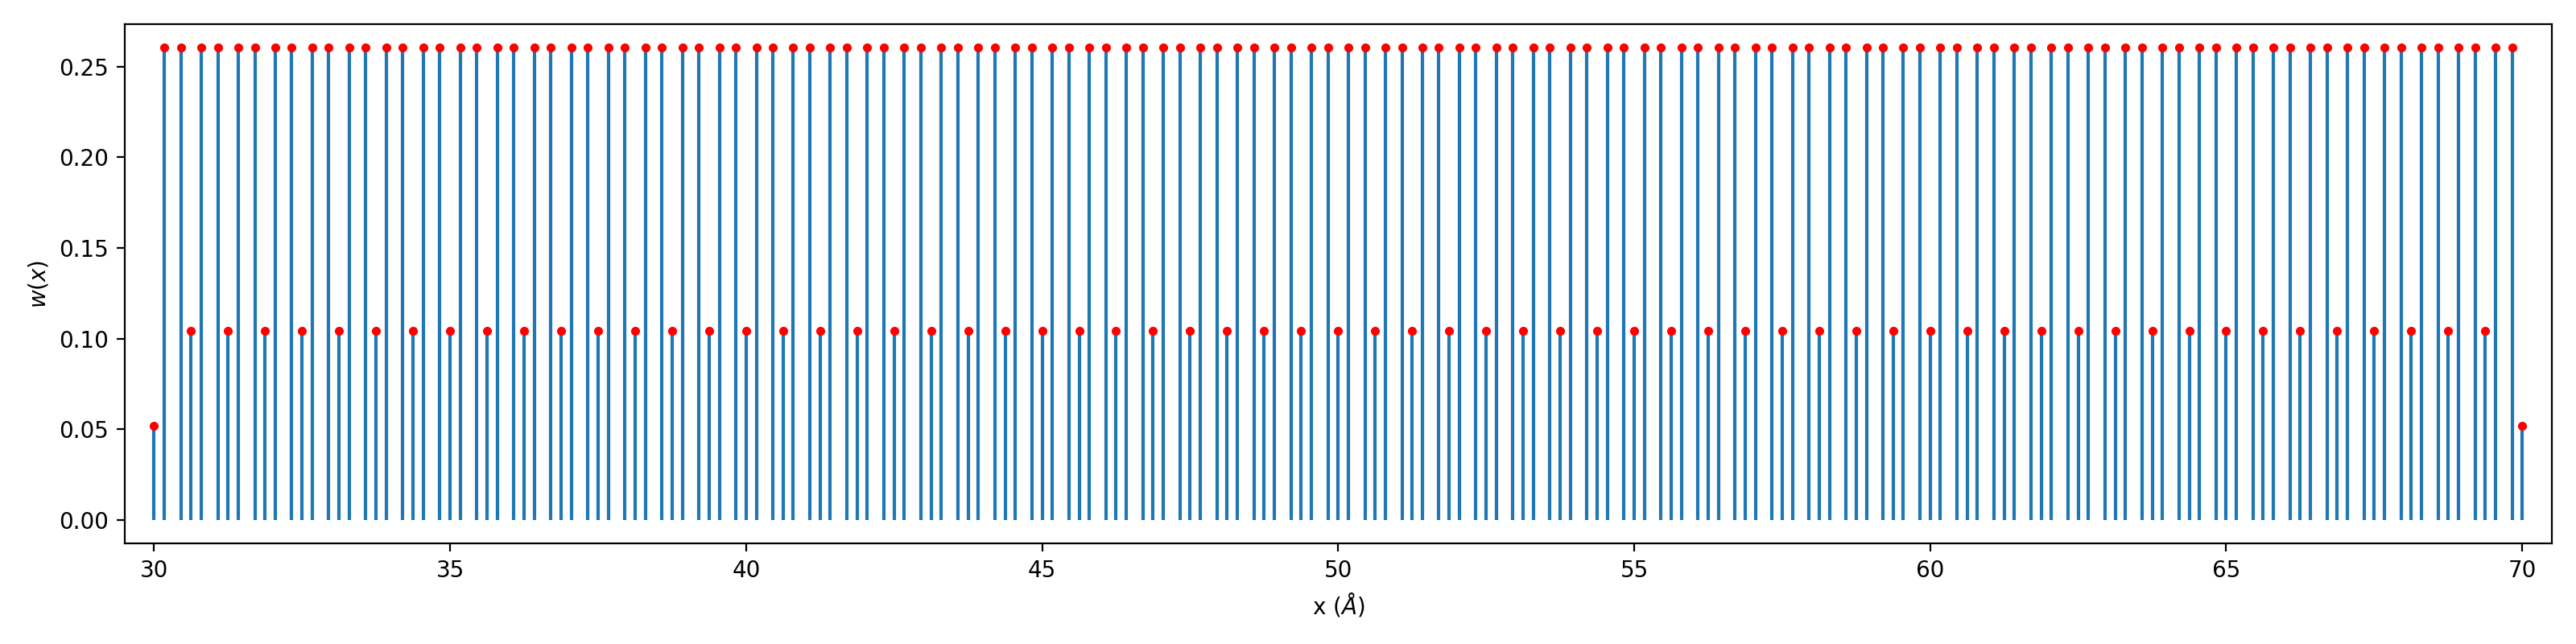
\includegraphics[scale=0.35]{ch3/weight_function.png}   
\end{center}
\end{definition}

\begin{definition}[Orthogonal]
We say that functions $f$ and $g$ are orthogonal if their inner product (equivalently, the value of this integral) is zero:
\begin{equation}
        \langle f,g\rangle _{w}=0.
\end{equation}
\end{definition}

\begin{definition}[Norm]
We define the norm with respect to this inner product as
\begin{equation}
        \|f\|_w = \sqrt{\langle f, f\rangle_w}
\end{equation}
\end{definition}

\section{Diagonalization of the operator}
\begin{definition}[Basis functions]
\begin{align}
        \psi^0_i(x) &= \rho_{\rm eq}(x) \phi^0_i(x) \\
        \phi^0_i(x) &= \sum_n c^0_n u_n(x).
\end{align}
\label{basisfunctions}
\end{definition}

\begin{definition}[Eigenvector matrix]
\begin{equation}
\Psi=
\begin{bmatrix}
\vert & \vert &  & \vert \\
\psi_1(x) & \psi_2(x) & \cdots & \psi_{N_v}(x) \\
\vert & \vert &  & \vert 
\end{bmatrix}
\end{equation}
\label{eigenvectormatrix}
Here, we get a set of orthonormal basis, $\langle \psi_i |$. The left part in the following part is 
\begin{equation}
        \Psi^T_{72\times 193}\Psi_{193 \times 72} = (\Psi^T\Psi)_{72 \times 72}
\end{equation}
The completeness relationship is actually can be seen by the blue points in the right part:
\begin{equation}
        \langle \psi_i(x),\psi_i(x)\rangle _{w} = \sum_{j=1}^{193}w(x_j)\psi_i(x_j)\psi_i(x_j)  = 1
\end{equation}
\begin{center}
        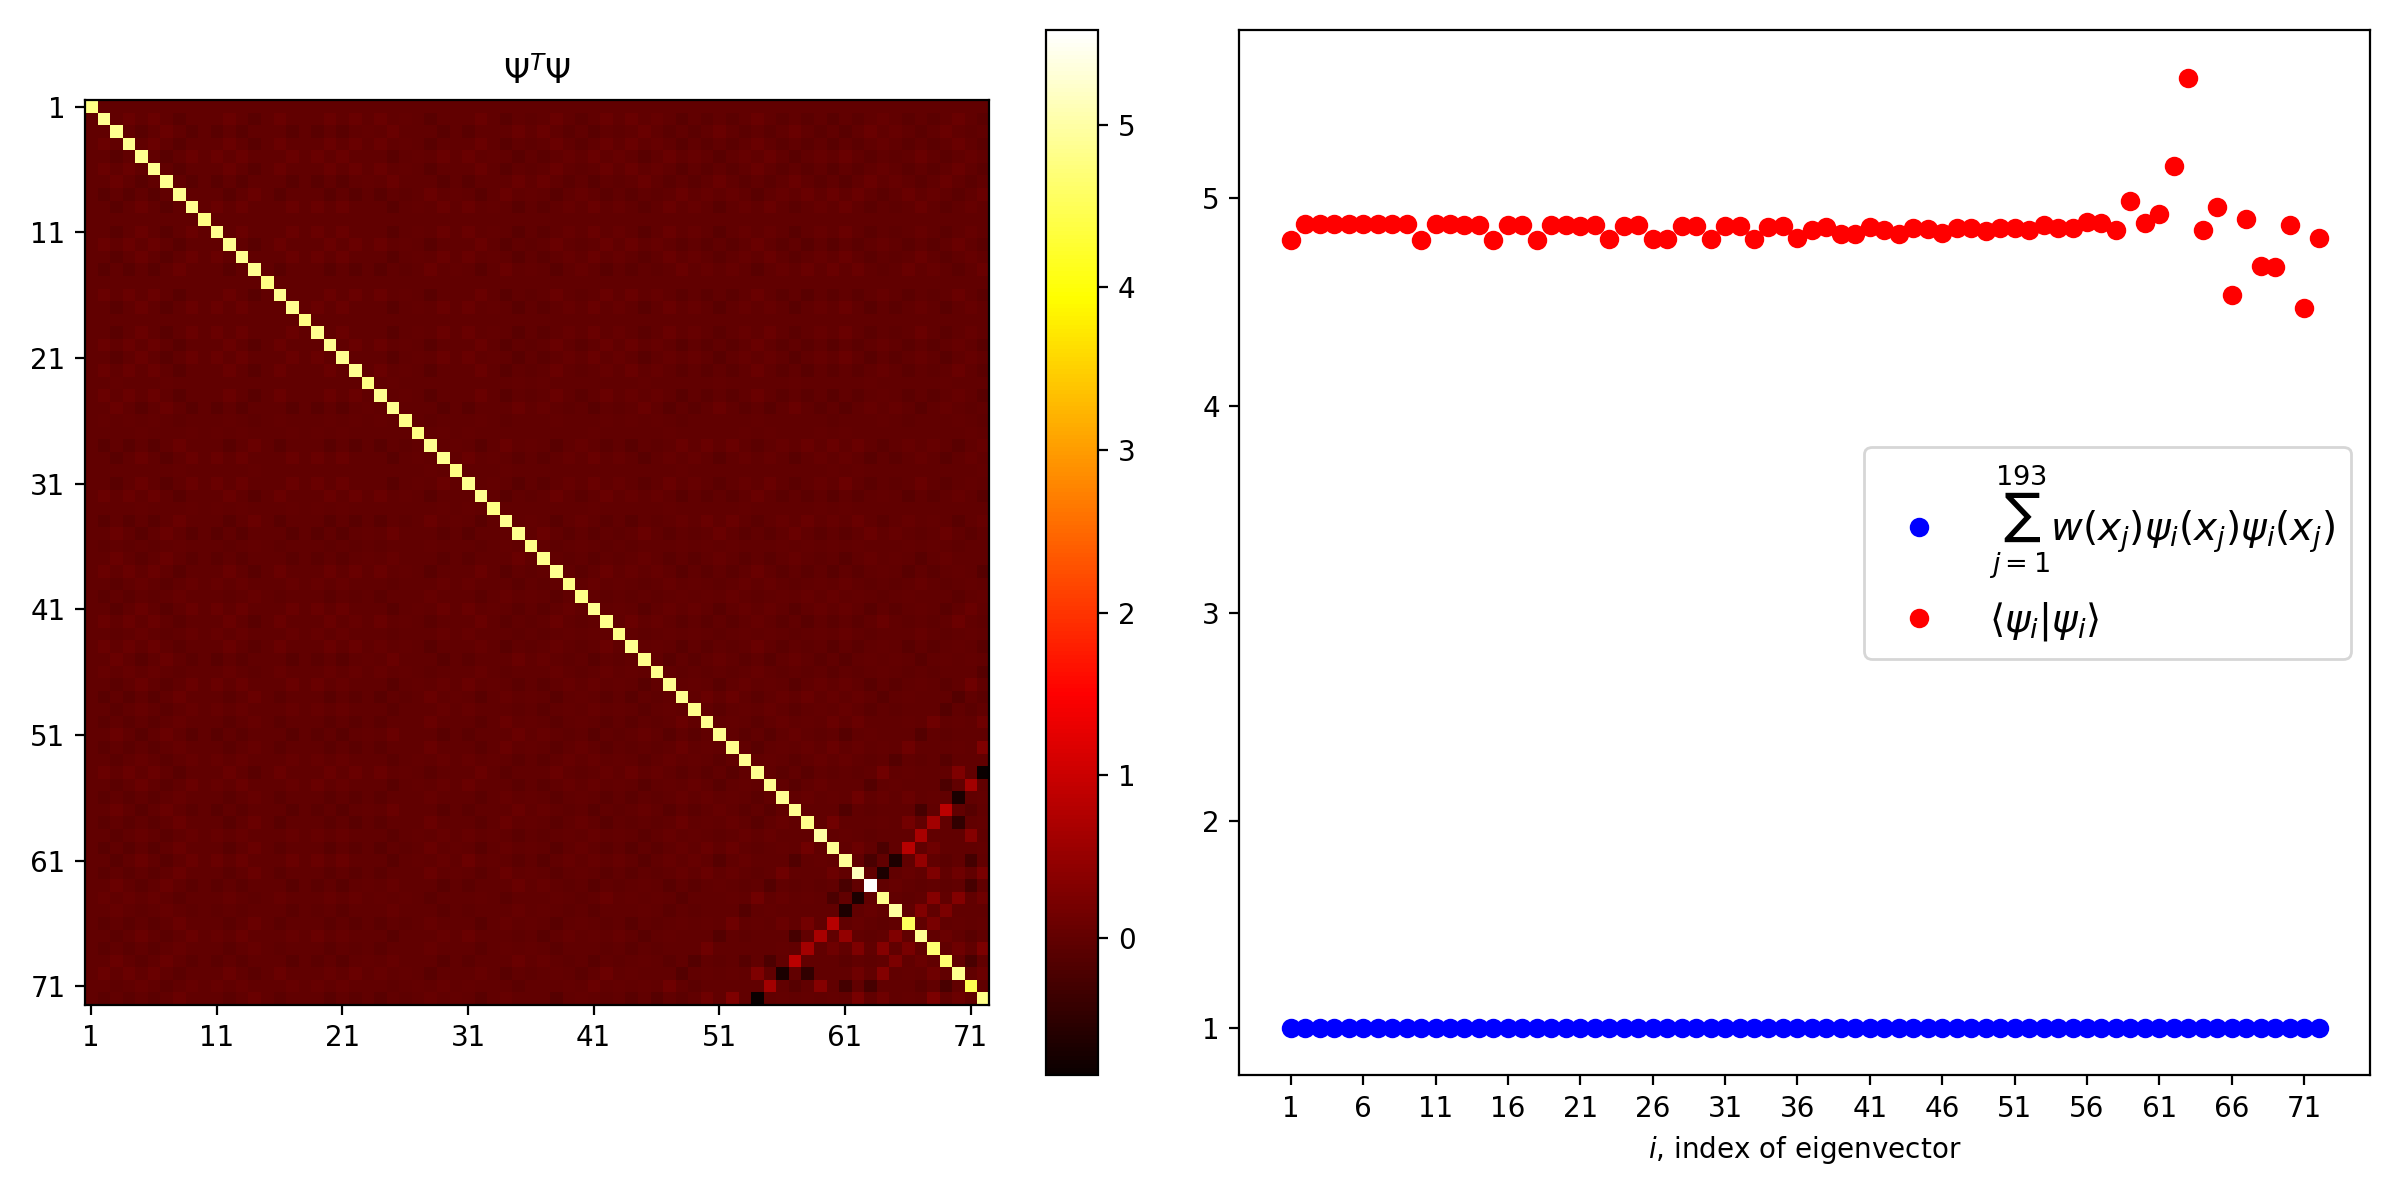
\includegraphics[scale=0.4]{ch3/eigenvec_matrix_complete.png}   
\end{center}
\end{definition}


%----------------------------------------------------------------------------------------
%	CHAPTER 4
%----------------------------------------------------------------------------------------
\chapterimage{head2.png} % Chapter heading image
\chapter{EM Algorithm}

\section{The General EM Algorithm}
\begin{definition}[The joint probability]
    \begin{equation}
        p(\textbf{x}, \textbf{y})= p(x_0)\prod_{t=1}^{T} p(x_{t}|x_{t-1}) p(y_t|x_t)
    \end{equation}
    \begin{center}
        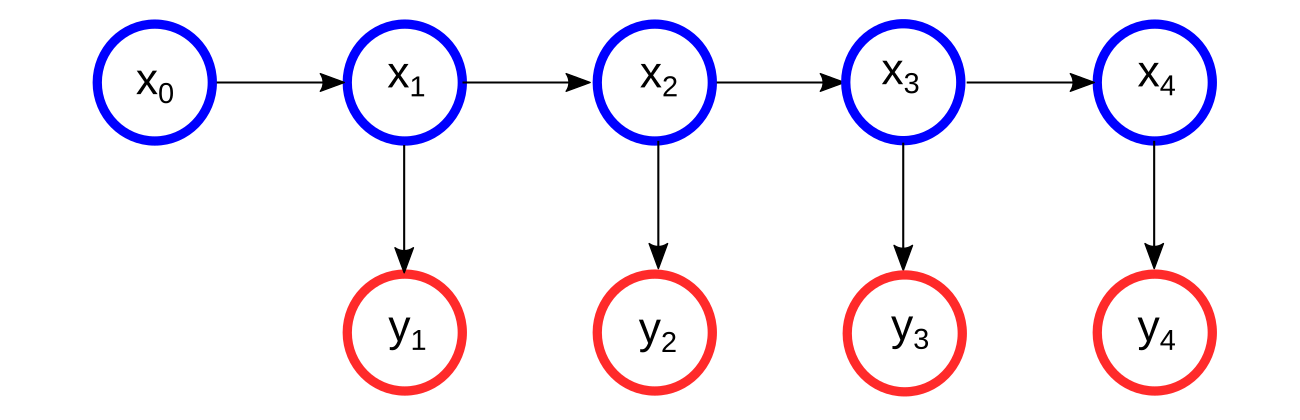
\includegraphics[scale=0.6]{ch2/four_states_ex.png}   
    \end{center}
In this example
    \begin{equation}
    \begin{split}
        p(\textbf{x}, \textbf{y})= &[p(x_0) p(x_1|x_0) p(y_1|x_1)] [p(x_2|x_1) p(y_2|x_2)]  [p(x_3|x_2) p(y_3|x_3)] \\
        &[p(x_4|x_3) p(y_4|x_4)]
    \end{split}
    \end{equation}
\end{definition}

\begin{definition}[The likelihood functional]
\begin{equation}
    L[\theta] = p(\textbf{y};\theta) = \int d\textbf{x}p(\textbf{x}, \textbf{y})
\end{equation}
\end{definition}

\begin{definition}[The log-likelihood functional]
\begin{equation}
    l[\theta] = \ln{(\int d\textbf{x}p(\textbf{x}, \textbf{y}))}
\end{equation}
\end{definition}

\begin{definition}[Solve Euler-Lagrange equation]
Maximization for the optimal parameter set requires taking derivatives of the log-likelihood functional and solves the resulting Euler-Lagrange equation:
\begin{equation}
        \frac{\partial l[\theta]}{\partial \theta} = \frac{\partial}{\partial \theta} \ln{(\int d\textbf{x}p(\textbf{x}, \textbf{y}))} = 0
\end{equation}
We can further get
\begin{equation}
    \frac{\partial l[\theta]}{\partial \theta} =  \frac{\partial \ln{L[\theta]}}{\partial \theta} = \frac{1}{L[\theta]}\frac{\partial L[\theta]}{\partial \theta}
\end{equation}
Because we need to do maximization according to previous step($k$), we want to solve the
following equation
\begin{equation}
    0 = \frac{\partial l^k[\theta]}{\partial \theta} = \frac{1}{L^k[\theta]}\frac{\partial L^k[\theta]}{\partial \theta}
\end{equation}
And we can express the likelihood functional as
\begin{equation}
    L^k[\theta] = p(\textbf{y}) = \sum_{\tau=0}^{T-1} \left<\alpha^k_{t_{\tau}}\right|  e^{-\textbf{H} \Delta t} \left|\beta^k_{t_{\tau+1}}\right>
\end{equation}
Therefore, the maximization problem becomes to solve
\begin{equation}
    0 =  \frac{\partial l^k[\theta]}{\partial \theta} = \frac{1}{L^k[\theta]} \sum_{\tau=0}^{T-1} \frac{\partial}{\partial \theta} \left<\alpha^k_{t_{\tau}}\right|  e^{-\textbf{H} \Delta t} \left|\beta^k_{t_{\tau+1}}\right>
\end{equation}
\end{definition}

\section{The expected log of the complete likelihood}
\begin{definition}[$\left<\alpha^k_{t_{0}}\right|  e^{-\textbf{H} \Delta t} \left|\beta^k_{t_{1}}\right>$]
\begin{equation}
    \left< \alpha_{t_0} | e^{-\textbf{H}\Delta t} | \beta_{t_1} \right> = \int p(x_0) p(x_1|x_0) p(y_2,y_3,y_4|x_1) dx_1= p(x_0,y_2,y_3,y_4)
\end{equation}
    \begin{center}
        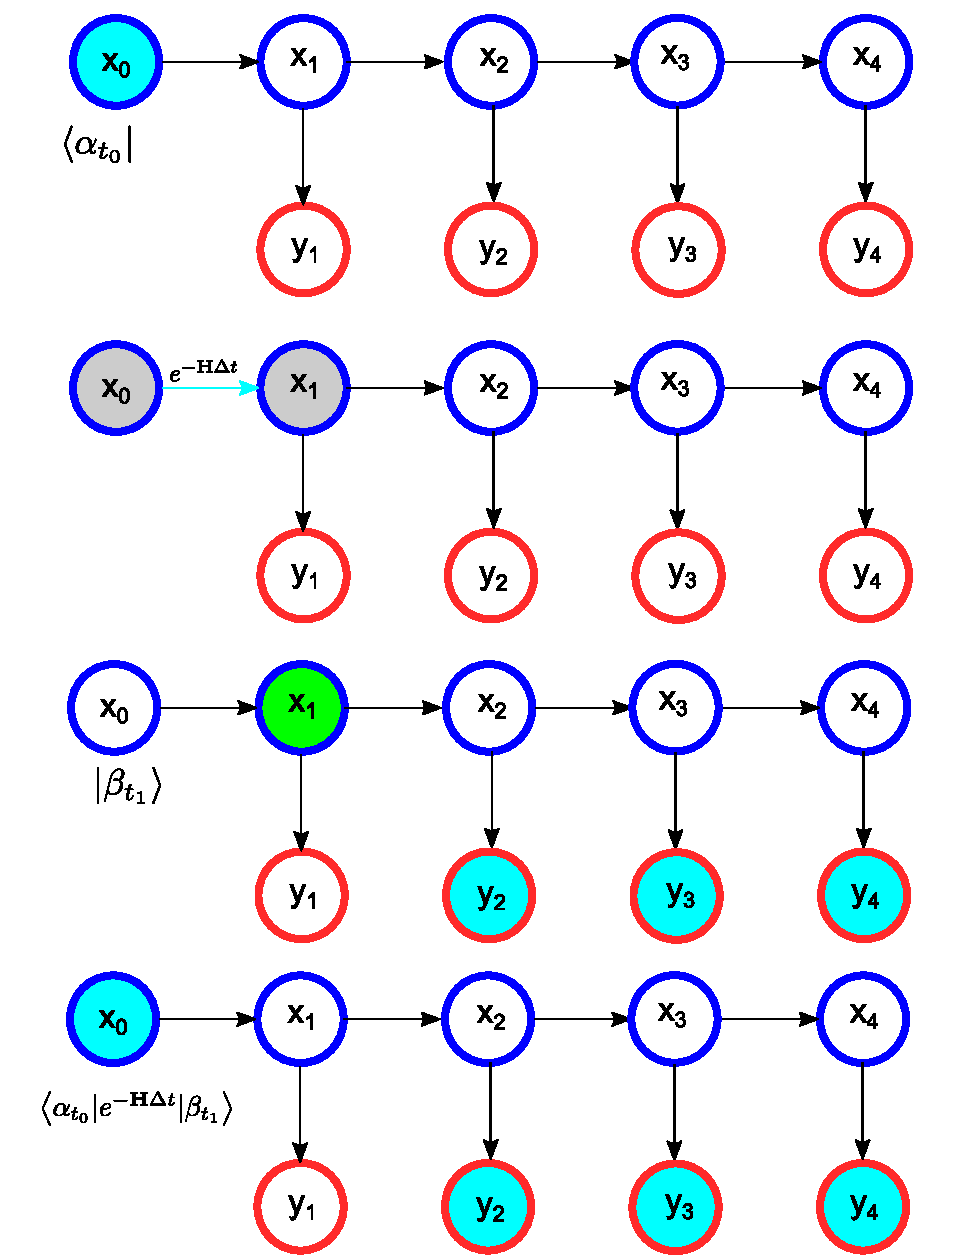
\includegraphics[scale=0.25]{ch4/alpha_t0_e_beta_t1.pdf}   
    \end{center}
\end{definition}

\begin{definition}[$\left<\alpha^k_{t_{1}}\right|  e^{-\textbf{H} \Delta t} \left|\beta^k_{t_{2}}\right>$]
\begin{equation}
    \left< \alpha_{t_1} | e^{-\textbf{H}\Delta t} | \beta_{t_2} \right> = \int p(x_1,y_1) p(x_2|x_1) p(y_3,y_4|x_2) dx_2= p(x_1,y_1,y_3,y_4)
\end{equation}
\begin{center}
    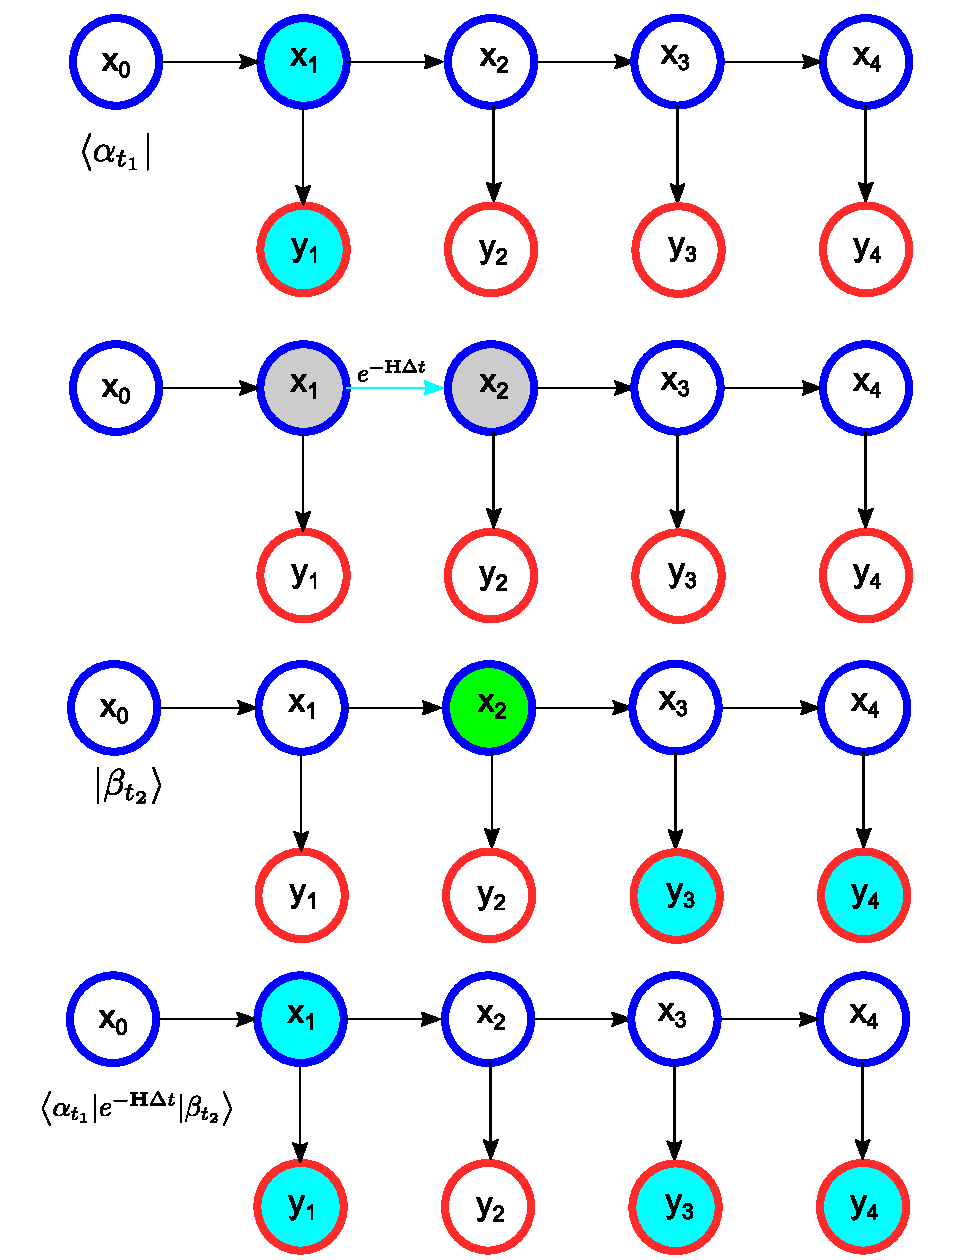
\includegraphics[scale=0.35]{ch4/alpha_t1_e_beta_t2.pdf}   
\end{center}
\end{definition}

\begin{definition}[$\left<\alpha^k_{t_{2}}\right|  e^{-\textbf{H} \Delta t} \left|\beta^k_{t_{3}}\right>$]
\begin{equation}
    \left< \alpha_{t_2} | e^{-\textbf{H}\Delta t} | \beta_{t_3} \right> = \int p(x_2,y_1,y_2) p(x_3|x_2) p(y_4|x_3) dx_3= p(x_2,y_1,y_2,y_4)
\end{equation}
\begin{center}
    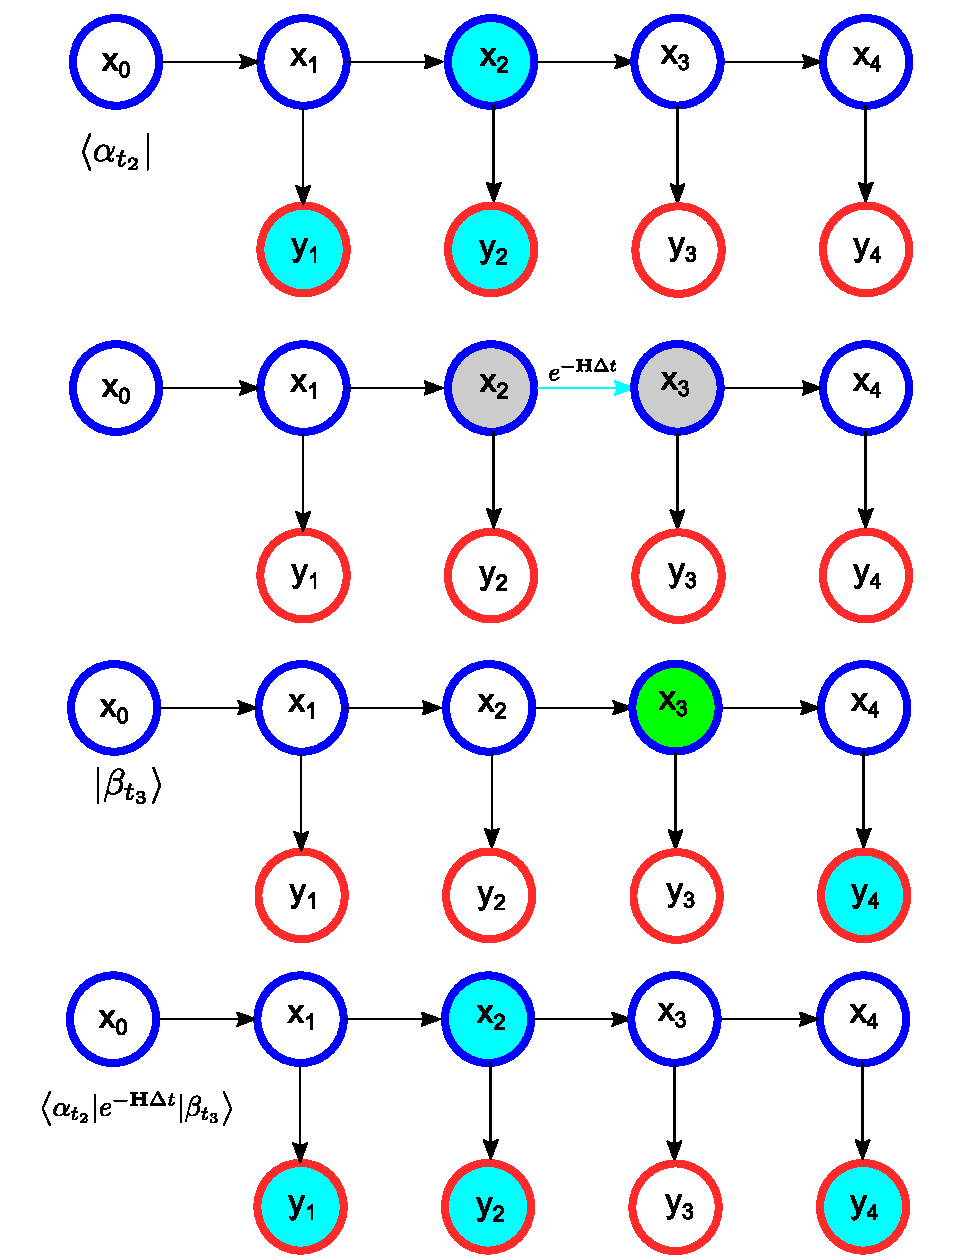
\includegraphics[scale=0.35]{ch4/alpha_t2_e_beta_t3.pdf}   
\end{center}
\end{definition}

\begin{definition}[$\left<\alpha^k_{t_{3}}\right|  e^{-\textbf{H} \Delta t} \left|\beta^k_{t_{4}}\right>$]
\begin{equation}
    \left< \alpha_{t_3} | e^{-\textbf{H}\Delta t} | \beta_{t_4} \right> = \int p(x_3,y_1,y_2,y_3) p(x_4|x_3) dx_4= p(x_3,y_1,y_2,y_3)
\end{equation}
\begin{center}
    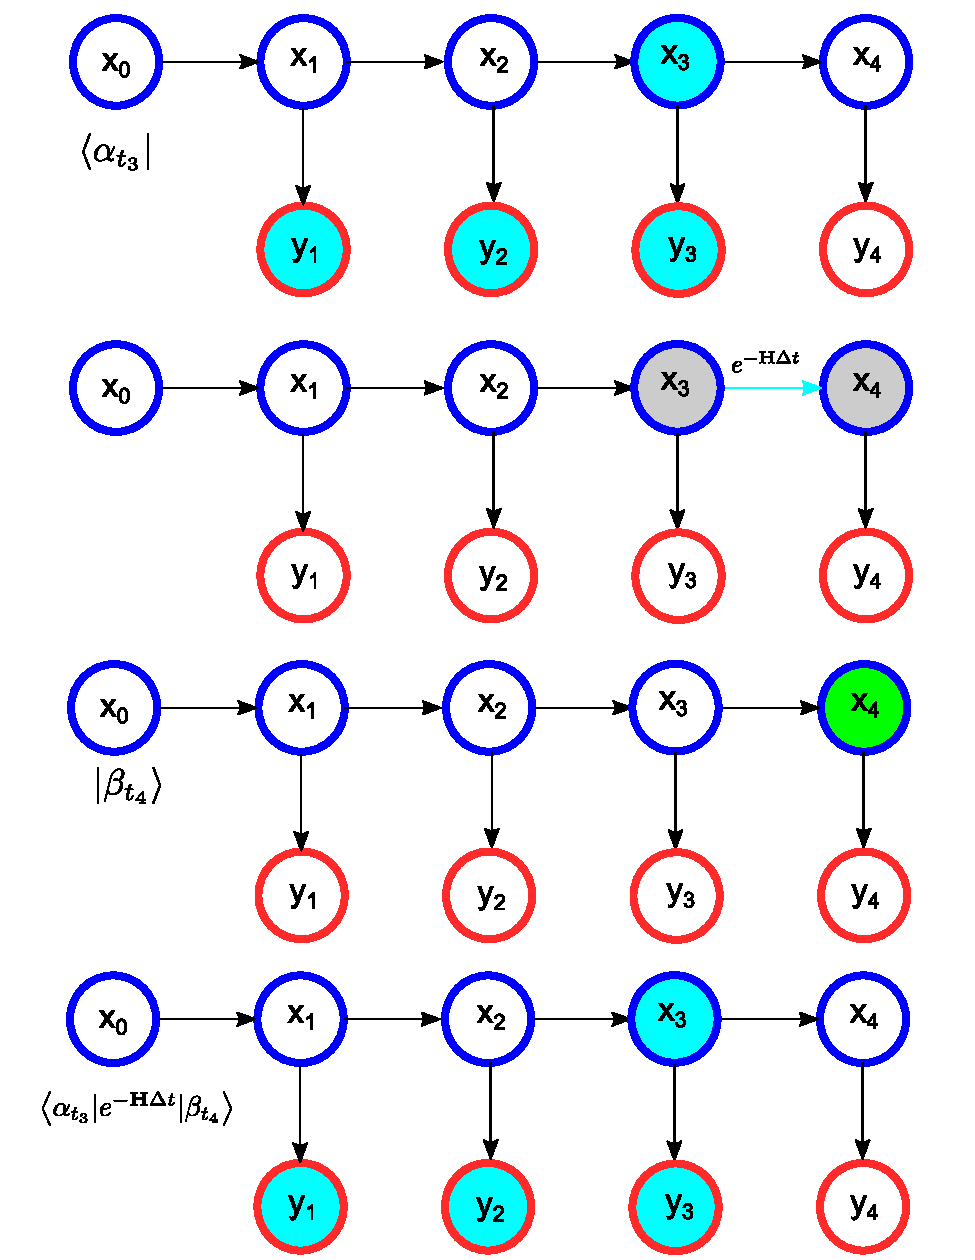
\includegraphics[scale=0.25]{ch4/alpha_t3_e_beta_t4.pdf}   
\end{center}
\end{definition}

\section{Update the equilibrium probability density}
\begin{definition}
    The basis functions in Def.(\ref{basisfunctions}) were used to update
\begin{align}
    p_{\rm eq}^{k+1}(x) &=\mathbb{E}^k_{X|Y} \left[ \delta(x-X) \right] \\
    &= p^k_{\rm{eq}}(x) \sum_{i,j} \mathbb{E}^k_{X|Y}[a_ib_j] \phi_i(x)\phi_j(x) \\
    &= \sum_{i,j} \psi_i(x) \mathbb{E}^k_{X|Y}[a_ib_j] \psi_j(x).
\end{align}
\end{definition}

\begin{definition}[Update from matrix multiplication]
\begin{align}
    p_{\rm eq}^{k+1}(x) = \mathrm{diag}(\Psi \mathbb{E}^k_{X|Y}[a_ib_j] \Psi^{\dagger})
\end{align}
\end{definition}

\begin{example}[$N_v=3$] In the matrix multiplication, I abbreviate $\mathbb{E}^k_{X|Y}[a_ib_j]$ as $a_ib_j$, and the grids are set like the bottom figure. We will show
\begin{align*}
    p_{\rm eq}^{k+1}(x) &=\sum_{i,j} \psi_i(x) \mathbb{E}^k_{X|Y}[a_ib_j] \psi_j(x) \\
    &= \mathrm{diag}(\Psi \mathbb{E}^k_{X|Y}[a_ib_j] \Psi^{\dagger})
\end{align*}
\begin{center}
    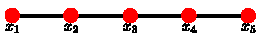
\includegraphics[scale=1.5]{ch4/ex1_grids.pdf}   
\end{center}
\begin{align*} 
&\Psi \mathbb{E}^k_{X|Y}[a_ib_j] \Psi^{\dagger} = \\
&\begin{bmatrix}
    \psi_1(x_1) & \psi_2(x_1) & \psi_3(x_1)  \\
    \psi_1(x_2) & \psi_2(x_2) & \psi_3(x_2) \\
    \psi_1(x_3) & \psi_2(x_3) & \psi_3(x_3)  \\
    \psi_1(x_4) & \psi_2(x_4) & \psi_3(x_4)  \\
    \psi_1(x_5) & \psi_2(x_5) & \psi_3(x_5)  
\end{bmatrix}
\begin{bmatrix}
    a_1 b_1 & a_1 b_2 & a_1 b_3  \\
    a_2 b_1 & a_2 b_2 & a_2 b_3 \\
    a_3 b_1 & a_3 b_2 & a_3 b_3
\end{bmatrix}
\begin{bmatrix}
    \psi_1(x_1) & \psi_1(x_2) & \psi_1(x_3) & \psi_1(x_4) & \psi_1(x_5) \\
    \psi_2(x_1) & \psi_2(x_2) & \psi_2(x_3) & \psi_2(x_4) & \psi_2(x_5) \\
    \psi_3(x_1) & \psi_3(x_2) & \psi_3(x_3) & \psi_3(x_4) & \psi_3(x_5) 
\end{bmatrix} \\
&=\begin{bmatrix}
    \sum_{i=1}^{3}a_i b_1 \psi_i(x_1) & \sum_{i=1}^{3}a_i b_2 \psi_i(x_1) & \sum_{i=1}^{3}a_i b_3 \psi_i(x_1) \\
    \sum_{i=1}^{3}a_i b_1 \psi_i(x_2) & \sum_{i=1}^{3}a_i b_2 \psi_i(x_2) & \sum_{i=1}^{3}a_i b_3 \psi_i(x_2) \\
    \sum_{i=1}^{3}a_i b_1 \psi_i(x_3) & \sum_{i=1}^{3}a_i b_2 \psi_i(x_3) & \sum_{i=1}^{3}a_i b_3 \psi_i(x_3) \\
    \sum_{i=1}^{3}a_i b_1 \psi_i(x_4) & \sum_{i=1}^{3}a_i b_2 \psi_i(x_4) & \sum_{i=1}^{3}a_i b_3 \psi_i(x_4) \\
    \sum_{i=1}^{3}a_i b_1 \psi_i(x_5) & \sum_{i=1}^{3}a_i b_2 \psi_i(x_5) & \sum_{i=1}^{3}a_i b_3 \psi_i(x_5) 
\end{bmatrix}\\
&\begin{bmatrix}
    \psi_1(x_1) & \psi_1(x_2) & \psi_1(x_3) & \psi_1(x_4) & \psi_1(x_5) \\
    \psi_2(x_1) & \psi_2(x_2) & \psi_2(x_3) & \psi_2(x_4) & \psi_2(x_5) \\
    \psi_3(x_1) & \psi_3(x_2) & \psi_3(x_3) & \psi_3(x_4) & \psi_3(x_5) 
\end{bmatrix}\\
&=
\begin{bmatrix}
\sum_{j=1}^{3} b_j \psi_j(x_1) \sum_{i=1}^{3}a_i \psi_i(x_1) &  \sum_{j=1}^{3} b_j \psi_j(x_2) \sum_{i=1}^{3}a_i \psi_i(x_1) &
\cdots & \sum_{j=1}^{3} b_j \psi_j(x_5) \sum_{i=1}^{3}a_i \psi_i(x_1) \\
\sum_{j=1}^{3} b_j \psi_j(x_1) \sum_{i=1}^{3}a_i \psi_i(x_2) &  \sum_{j=1}^{3} b_j \psi_j(x_2) \sum_{i=1}^{3}a_i \psi_i(x_2) &
\cdots & \sum_{j=1}^{3} b_j \psi_j(x_5) \sum_{i=1}^{3}a_i \psi_i(x_2) \\
\sum_{j=1}^{3} b_j \psi_j(x_1) \sum_{i=1}^{3}a_i \psi_i(x_3) &  \sum_{j=1}^{3} b_j \psi_j(x_2) \sum_{i=1}^{3}a_i \psi_i(x_3) &
\cdots & \sum_{j=1}^{3} b_j \psi_j(x_5) \sum_{i=1}^{3}a_i \psi_i(x_3) \\
\sum_{j=1}^{3} b_j \psi_j(x_1) \sum_{i=1}^{3}a_i \psi_i(x_4) &  \sum_{j=1}^{3} b_j \psi_j(x_2) \sum_{i=1}^{3}a_i \psi_i(x_4) &
\cdots & \sum_{j=1}^{3} b_j \psi_j(x_5) \sum_{i=1}^{3}a_i \psi_i(x_4) \\
\sum_{j=1}^{3} b_j \psi_j(x_1) \sum_{i=1}^{3}a_i \psi_i(x_5) &  \sum_{j=1}^{3} b_j \psi_j(x_2) \sum_{i=1}^{3}a_i \psi_i(x_5) &
\cdots & \sum_{j=1}^{3} b_j \psi_j(x_5) \sum_{i=1}^{3}a_i \psi_i(x_5)
\end{bmatrix}
\end{align*}
\end{example}

\section{EM Test}
\begin{center}
    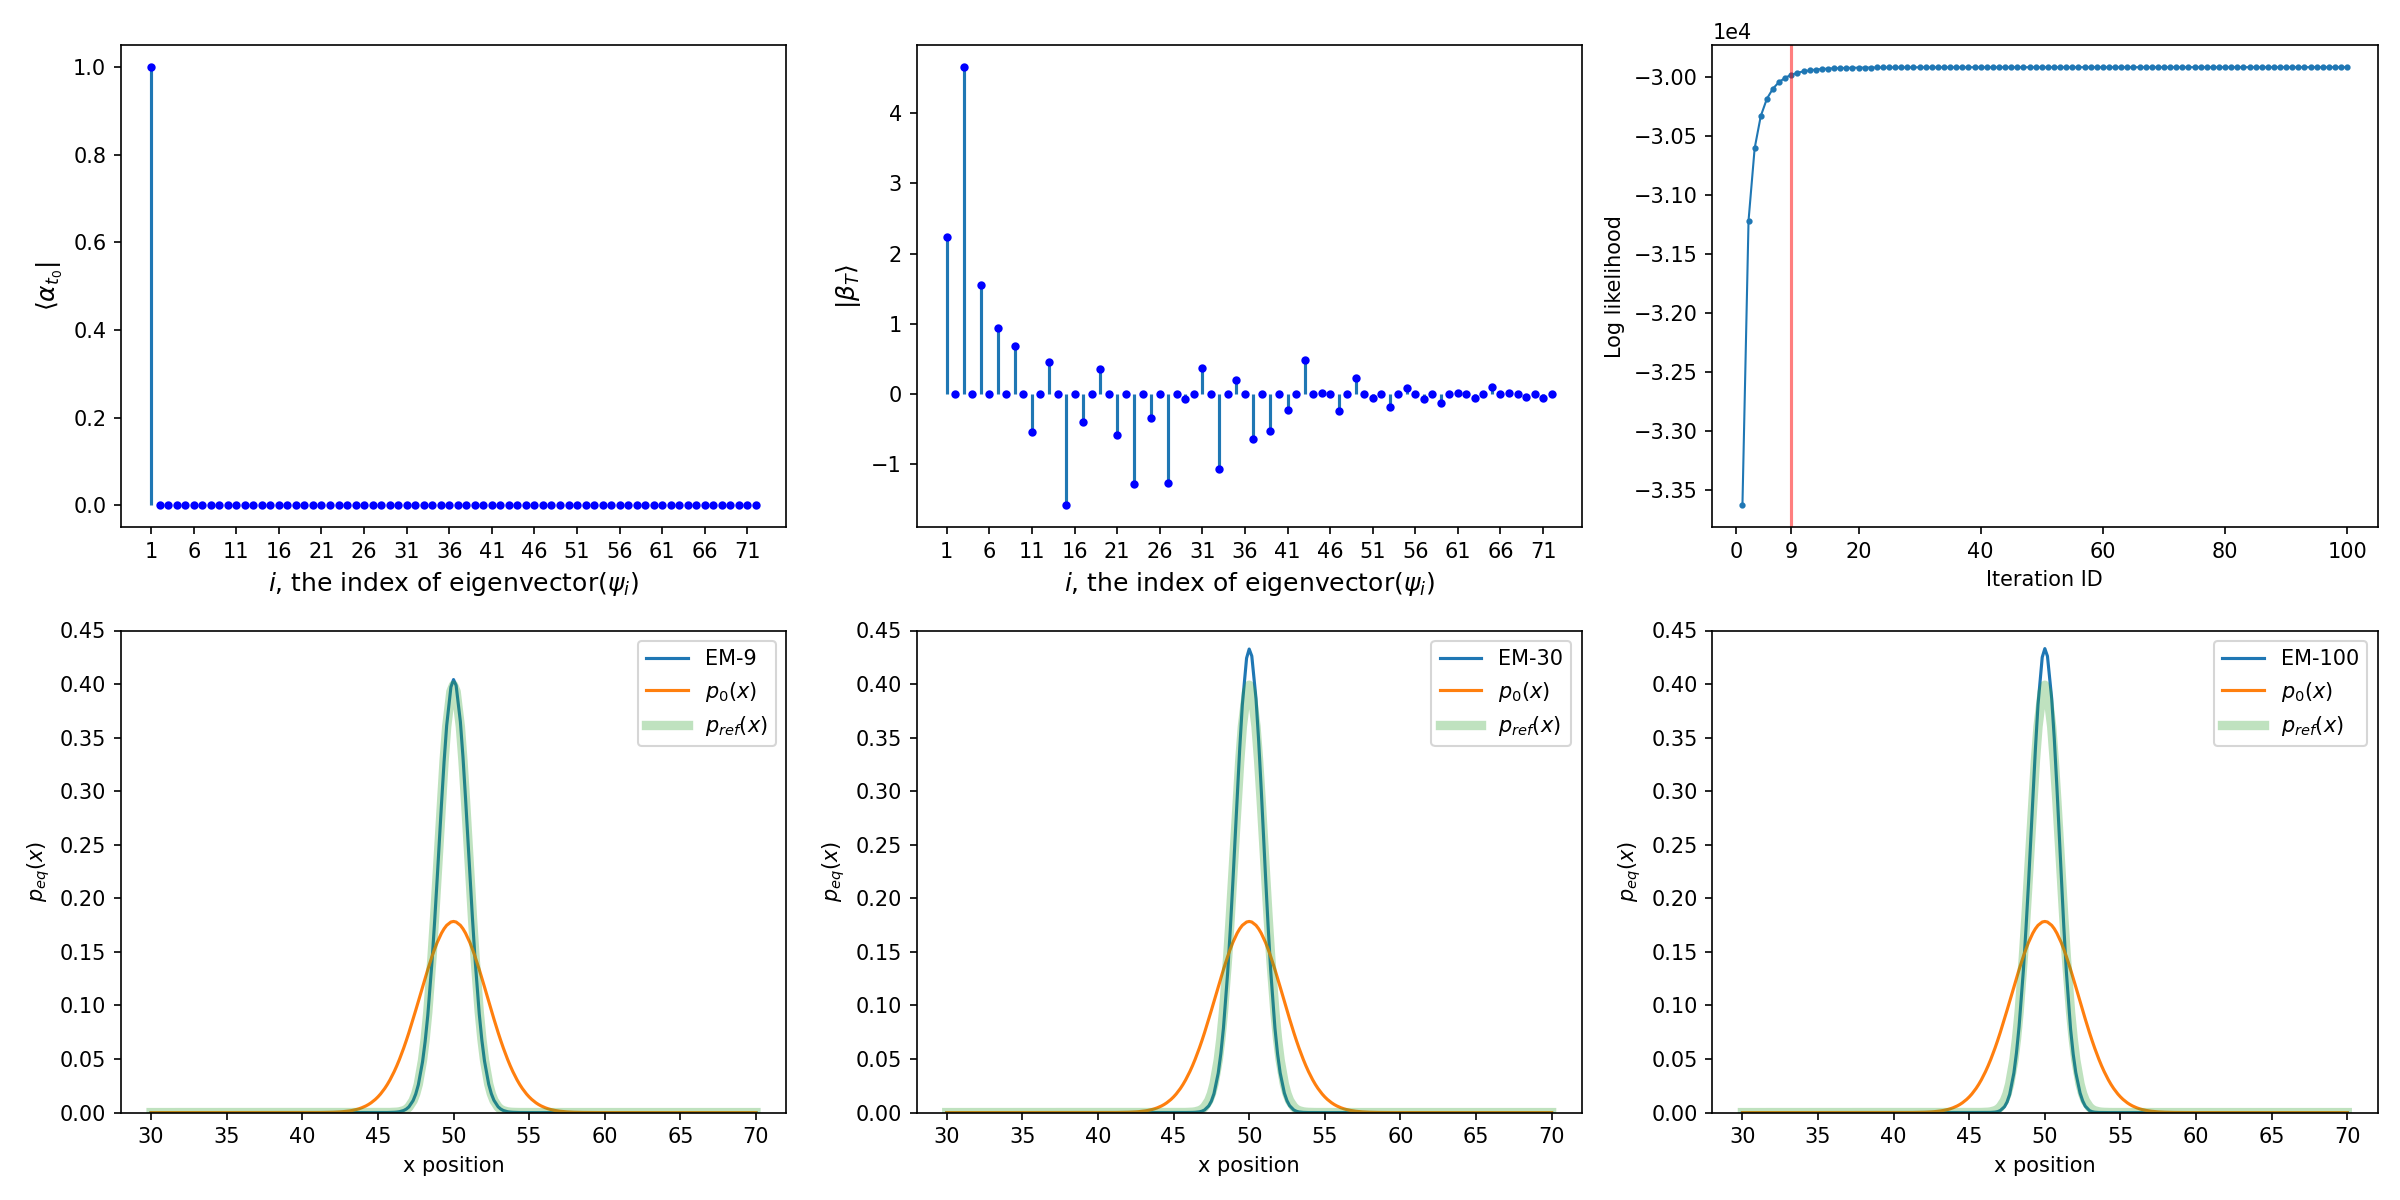
\includegraphics[scale=0.36]{ch4/forward_backward_v2.png}   
\end{center}

\subsection{Initial Guess Test}
\begin{center}
    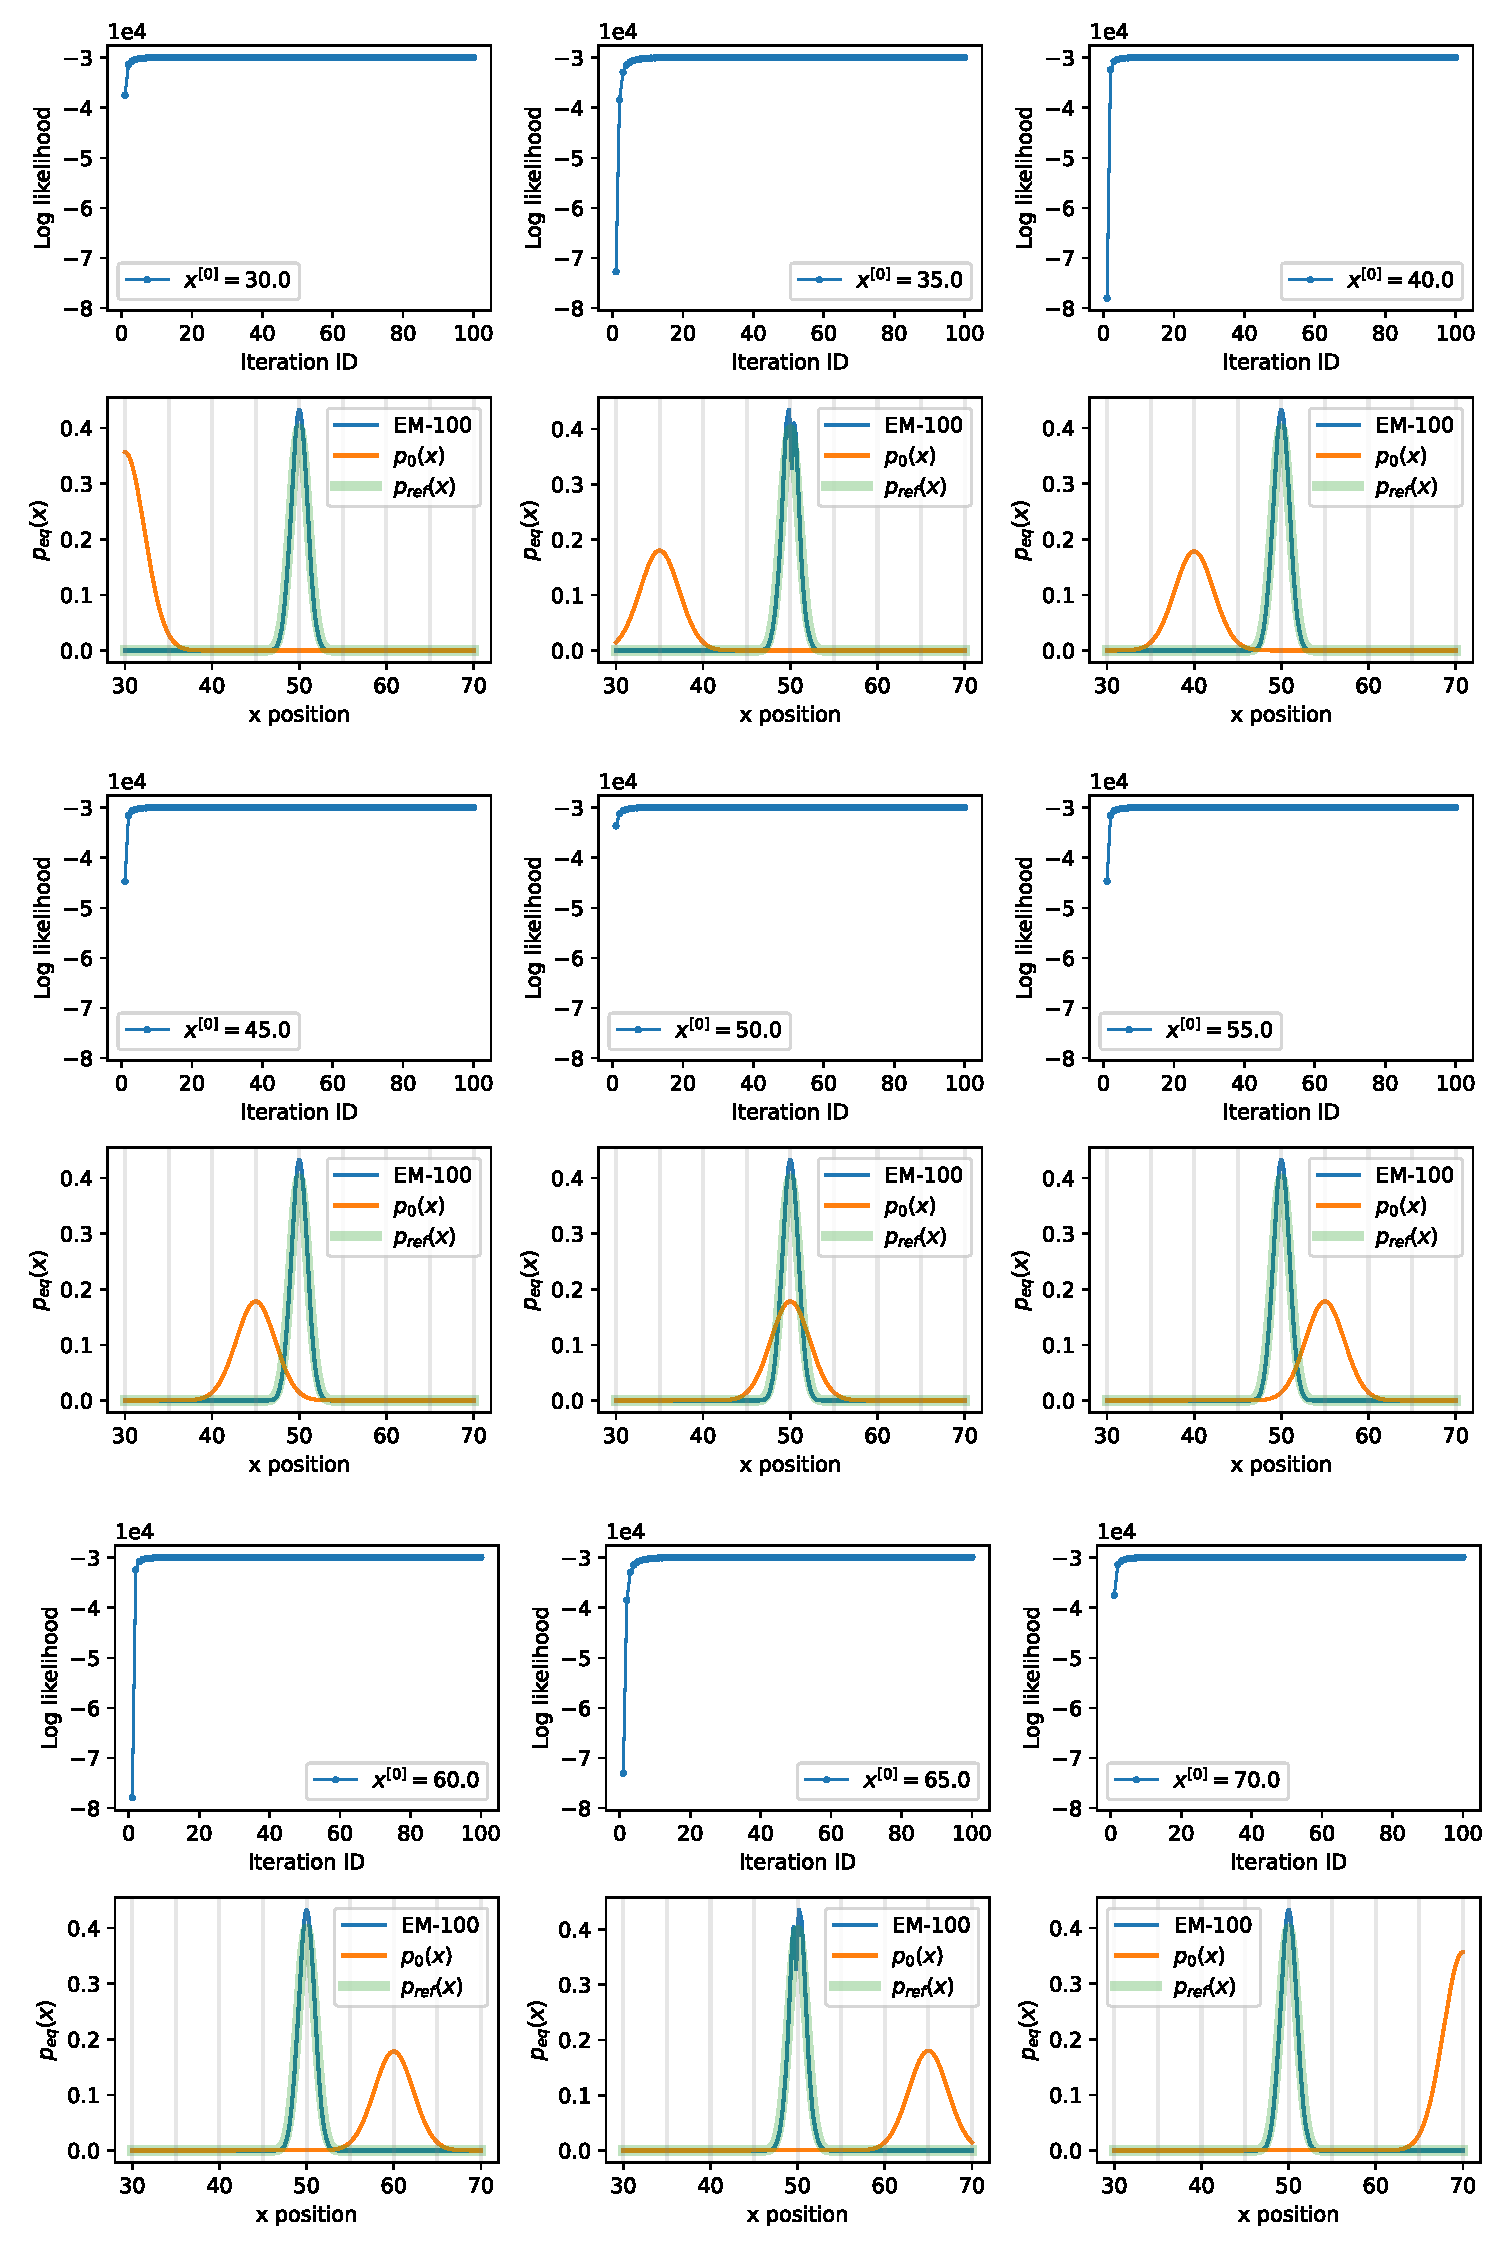
\includegraphics[scale=0.55]{ch4/initial_guess_test.pdf}   
\end{center}

\subsection{Troubleshooting: Double Peak}
\begin{center}
    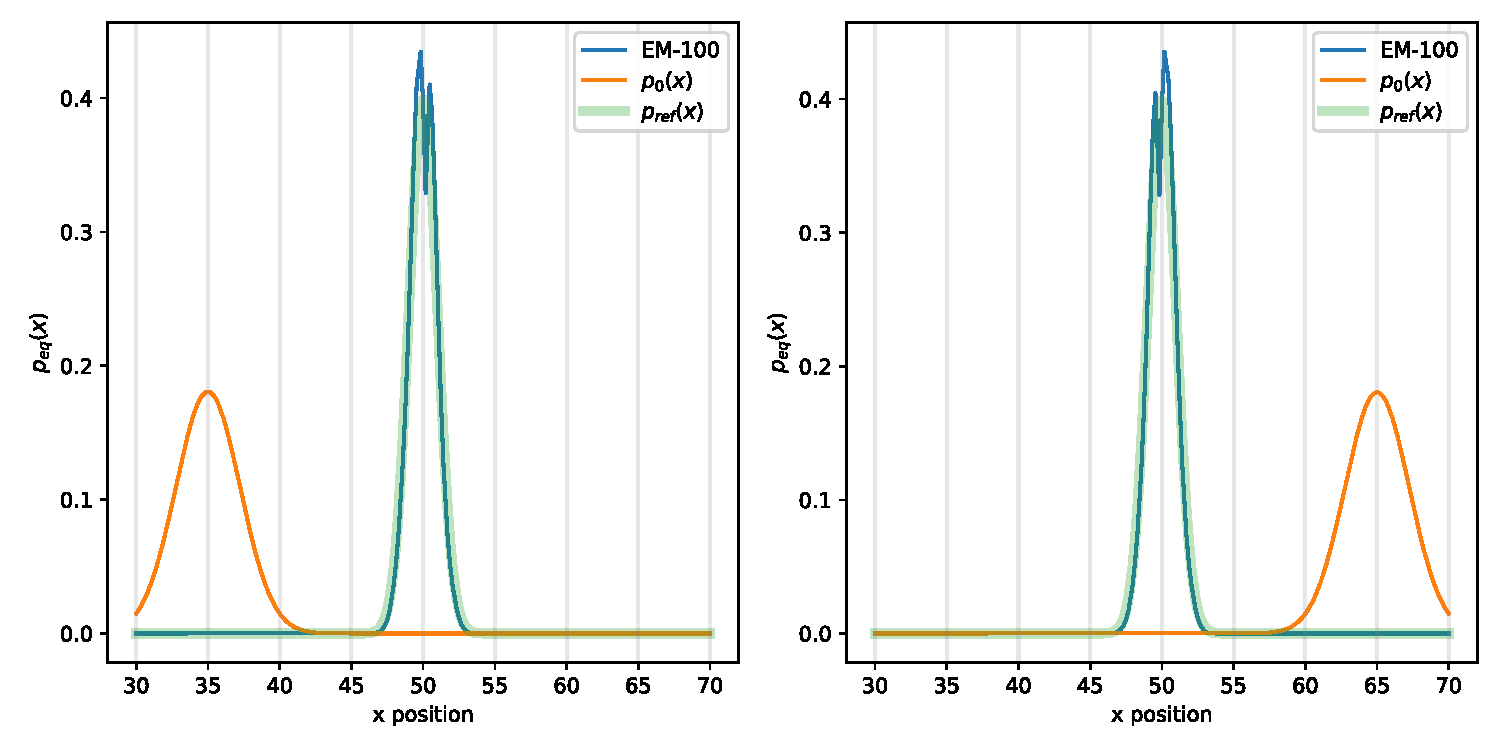
\includegraphics[scale=0.55]{ch4/double_peak_problem.pdf}   
\end{center}
\subsubsection{Step 1: Detect abrupt change}
\begin{itemize}
    \item Use finite difference to get $\frac{d p^{[k]}_{eq}(x)}{dx}$ and $\frac{d^2 p^{[k]}_{eq}(x)}{dx^2}$
    \item If $|\frac{d^2 p_{eq}(x)}{dx^2}|>1$, put the point into the list storing "change points"
    \item If $\text{Number}(\text{Change points}) > 0$, do smoothing. Else: no smooth 
\end{itemize}
\begin{center}
    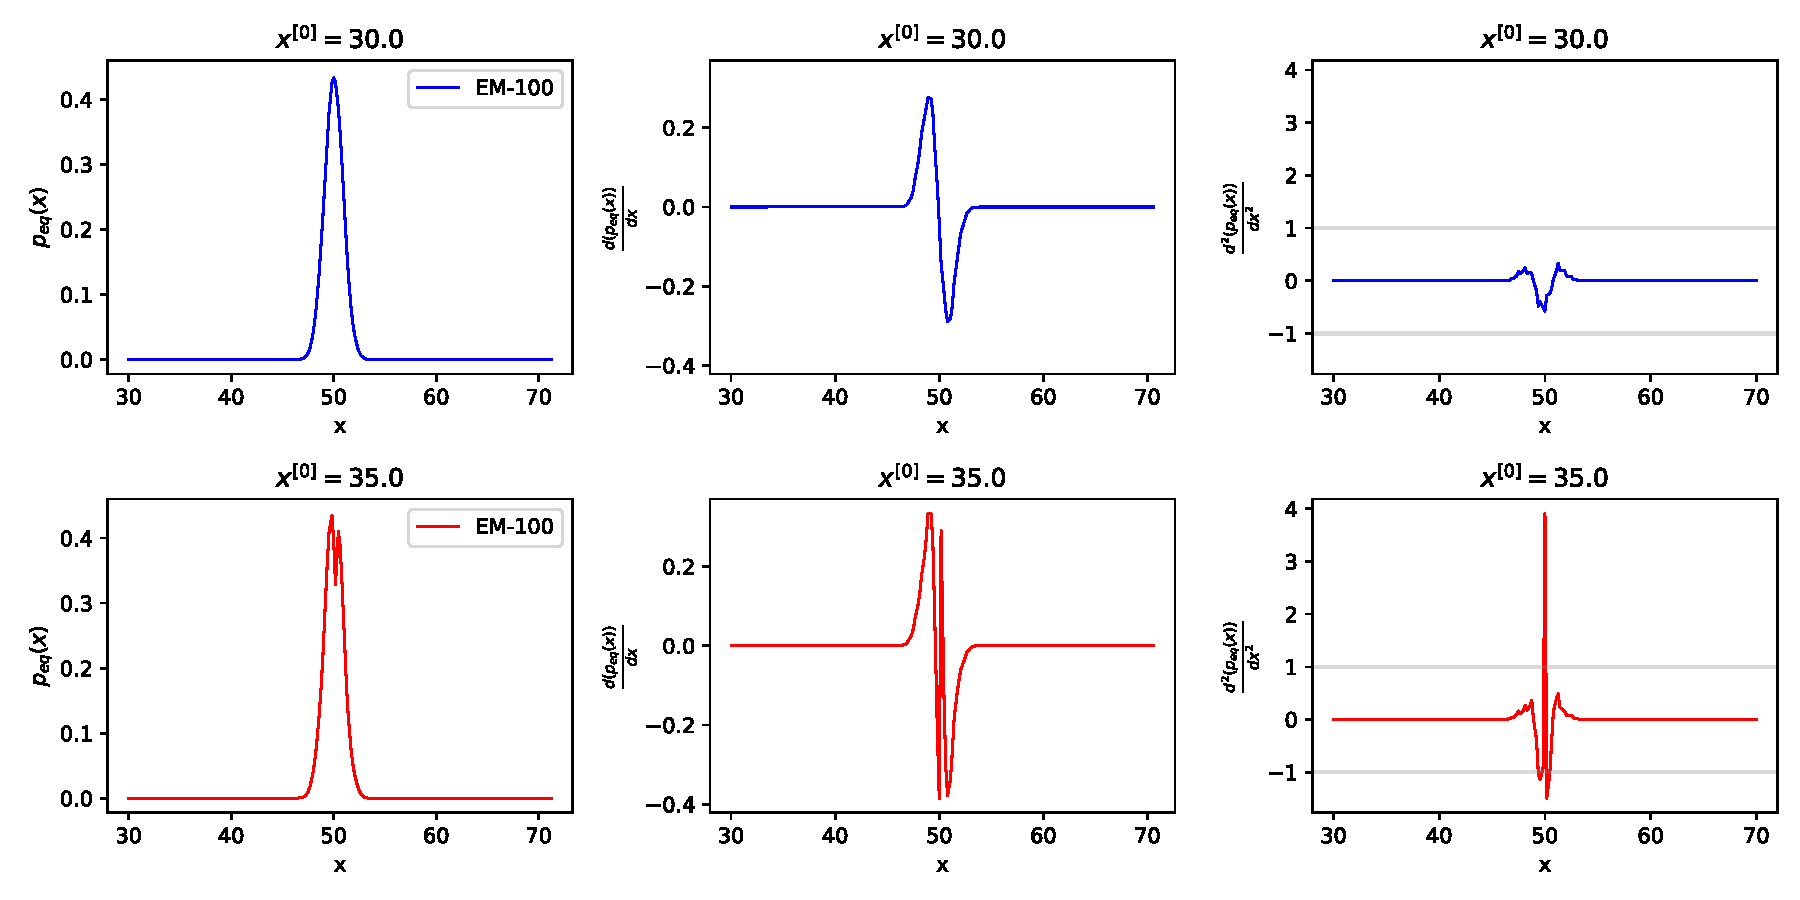
\includegraphics[scale=0.4]{ch4/double_peak_problem_derivative.pdf}   
\end{center}
\begin{center}
    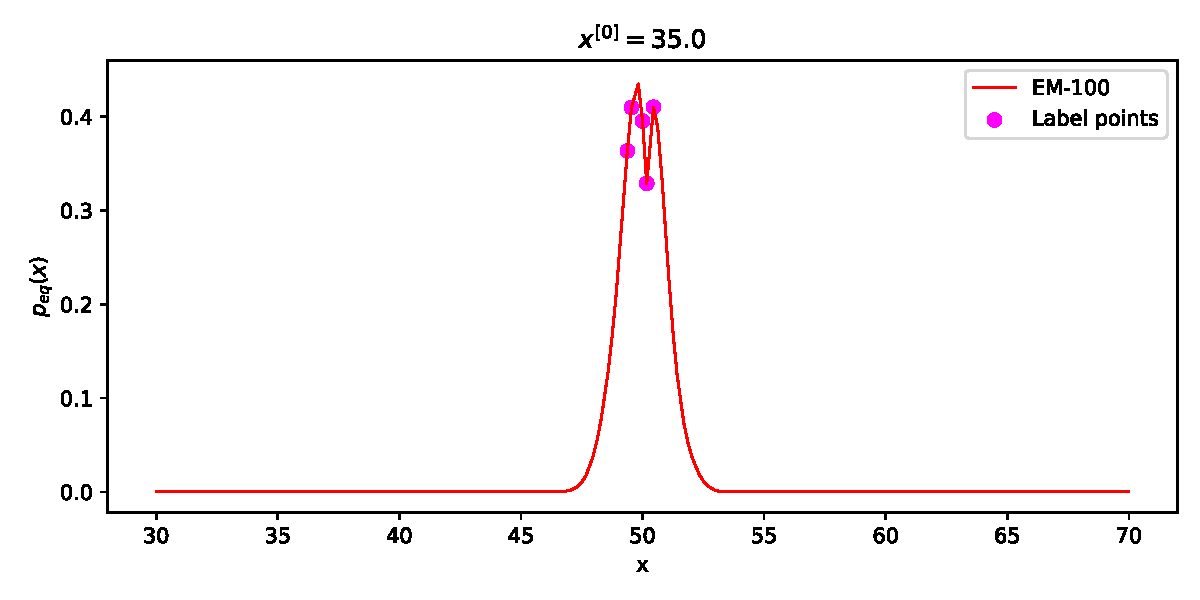
\includegraphics[scale=0.5]{ch4/abrupt_detect.pdf}   
\end{center}

\subsubsection{Step 2: Smoothing}
BBB
\subsubsection{Result}



\end{document}